\documentclass[a4paper]{article}

% CJK support: prefer ctex, fallback to XeTeX native line breaking
\IfFileExists{ctex.sty}{
  \usepackage[fontset=fandol]{ctex}
}{
  \usepackage{fontspec}
  \XeTeXlinebreaklocale "zh"
  \XeTeXlinebreakskip = 0pt plus 1pt
  \IfFontExistsTF{Songti SC}{\setmainfont{Songti SC}}{%
    \IfFontExistsTF{Noto Serif CJK SC}{\setmainfont{Noto Serif CJK SC}}{}%
  }
  \IfFontExistsTF{Heiti SC}{\setsansfont{Heiti SC}}{%
    \IfFontExistsTF{Noto Sans CJK SC}{\setsansfont{Noto Sans CJK SC}}{}%
  }
}

% Basic packages
\usepackage{amsmath, amssymb}
\usepackage{graphicx}
\usepackage[margin=2.5cm]{geometry}
\emergencystretch=3em
\usepackage[most]{tcolorbox}
\usepackage{etoolbox}
\usepackage{listings}
\usepackage{hyperref}
\hypersetup{hidelinks,pdftitle={南京大学生成式软件工程第10讲：软件的演化（航母是怎么造出来的）},pdfauthor={lecture-to-notes}}
\usepackage{booktabs}
\usepackage{subcaption}
\usepackage{float}
\usepackage{tikz}
\IfFileExists{pgfplots.sty}{
    \usepackage{pgfplots}
    \pgfplotsset{compat=1.18}
}{}

% ===== Highlight boxes =====
\newtcolorbox{knowledgebox}[1]{
    enhanced, colback=black!2!white, colframe=black!65, colbacktitle=black!65,
    coltitle=white, fonttitle=\bfseries, title=#1, attach boxed title to top left={yshift=-2mm, xshift=2mm},
    boxrule=1pt, sharp corners
}

\newtcolorbox{importantbox}[1]{
    enhanced, colback=red!3!white, colframe=red!45!black, colbacktitle=red!45!black,
    coltitle=white, fonttitle=\bfseries, title=#1, sharp corners
}

\newtcolorbox{warningbox}[1]{
    enhanced, colback=red!5!white, colframe=red!75!black, colbacktitle=red!75!black,
    coltitle=white, fonttitle=\bfseries, title=#1, sharp corners
}

% ===== Code listings =====
\lstset{
    basicstyle=\ttfamily\small,
    keywordstyle=\color{blue},
    stringstyle=\color{red!60!black},
    commentstyle=\color{green!60!black},
    breaklines=true,
    frame=single,
    numbers=left,
    numberstyle=\tiny\color{gray},
    captionpos=b,
    extendedchars=false
}

% ===== Figure provenance and unit macros =====
\newcommand{\vtag}{\protect\footnotemark}
\newcommand{\srcnote}[1]{\footnotetext{视频画面时间区间：#1。若为裁剪图，时间区间仍对应原视频画面。}}
\newcommand{\degC}{\ensuremath{^{\circ}\mathrm{C}}}
\newcommand{\um}{\ensuremath{\mu\mathrm{m}}}
\newcommand{\nm}{\ensuremath{\mathrm{nm}}}
\newcommand{\angstrom}{\ensuremath{\text{\AA}}}

% ===== Front-page metadata =====
\newcommand{\notetitle}{软件的演化（航母是怎么造出来的）}
\newcommand{\notesubtitle}{南京大学生成式软件工程 · 第 10 讲}
\newcommand{\noteauthors}{中文课程讲义 · lecture-to-notes}
\newcommand{\notedate}{2026 年 10 月 27 日}
\newcommand{\videochannel}{蒋炎岩主讲 / 绿导师原谅你了上传}
\newcommand{\videopublishdate}{20261027}
\newcommand{\videoduration}{99 分 54 秒}
\newcommand{\videourl}{https://www.bilibili.com/video/BV1Guxu6EERa/}
\newcommand{\videocoverpath}{cover.jpg}

\begin{document}

% ===== Title page =====
\begin{titlepage}
\centering
{\Large 课程笔记\par}
\vspace{1.2cm}
{\huge\bfseries \notetitle\par}
\ifdefempty{\notesubtitle}{}{
\vspace{0.3cm}
{\large \notesubtitle\par}
}
\vspace{0.5cm}
{\large \noteauthors\par}
\vspace{0.3cm}
{\large \notedate\par}
\vspace{1.0cm}

\ifdefempty{\videocoverpath}{
{\small 请在生成笔记时填入视频封面图的本地路径。\par}
}{
\includegraphics[width=0.82\textwidth,height=0.40\textheight,keepaspectratio]{\videocoverpath}\par
}

\vfill
\begin{tcolorbox}[width=0.9\textwidth, colback=black!2!white, colframe=black!60, sharp corners]
\textbf{视频作者/频道}：\videochannel\par
\textbf{发布日期}：\videopublishdate\par
\textbf{视频时长}：\videoduration\par
\textbf{视频链接}：\ifdefempty{\videourl}{待填写}{\url{\videourl}}\par
\end{tcolorbox}
\end{titlepage}

% ===== Executive Summary =====
\newpage
\section*{执行摘要与核心脉络}

本讲义对应南京大学 2026 年《生成式软件工程》（Generative Software Engineering）第 10 讲《软件的演化（航母是怎么造出来的）》，由蒋炎岩老师主讲。在上一讲将 DeepSeek Harness（\texttt{dsh}）剖析为智能体时代的“微内核操作系统”之后，本讲把视角从静态架构推向\textbf{时间维度（Evolution over Time）}，系统回答了一个困扰软件工程与人工智能的核心问题：\textbf{一个极其复杂的工业巨兽（无论是航空母舰还是数万次提交的现代软件系统），究竟是如何在历史长河中一步步演化出来的？在 AI 已经能轻松解决单点编码任务（SWE-bench）的今天，人类工程师真正的护城河——架构品味（Taste）与设计空间跳跃——又该如何锤炼与度量？}

全讲围绕八个层层递进的核心篇章展开：
\begin{enumerate}
    \item \textbf{日常震惊与理论计算机的“平坦”幻觉}：从 OpenAI 宣称给出 $k$-CNF 精确计数的亚指数时间算法、动摇指数时间假说（ETH）谈起，剖析人类科学工具的局限——多项式时间（\texttt{PTIME}）将 $n^2$ 与 $n$ 的 100次方混为一谈，纯粹是为了迁就归约与函数复合闭包（$P \circ P = P$）；正如生物分类树（Tree of Life）在微生物水平基因转移下退化为图结构，人类之所以能发现物理定律与 Scaling Law，是因为“我们刚好站在对称性与守恒律支配的平坦区域”。
    \item \textbf{教育循环松动与 AI Trajectory 简历革命}：当 \texttt{Senior + Agent > Junior} 打破“家庭投资—大学培养—企业购买”的闭环，且 Spence（1973）学历信号与静态项目成品均因 AI 代写而失真时，本讲提出以不可伪造的\textbf{人机交互轨迹（AI Trajectory）}作为新一代能力证明——面试官只需随机抽查某一天（例如 2026年 3 月 10 日）的交互日志，观察候选人何时拒绝 AI、依据什么证据推翻假设、第二次遇到同类问题时是否收敛得更快，即可精准还原其真实工程潜力。
    \item \textbf{航母是怎么造出来的——四代舰船的百年演化}：从 2019年圣地亚哥参访 1945年下水的中途岛号航空母舰（USS Midway，CV-41）切入，揭示复杂工程并非一蹴而就，而是每次在既有状态上叠加一个可验证的增量 $\Delta$：从 1492年哥伦布驾驭风力的圣玛丽亚号（Santa Maria），到 1811年（1812年首航抵达）把蒸汽动力装进船体的新奥尔良号（New Orleans）明轮汽船，再到 1913年运煤船 USS Jupiter 于 1922年拆掉运煤桁架、铺设木质飞行甲板改装为美国海军第一艘航母兰利号（USS Langley，CV-1），最终演进到 1945年围绕高密度航空作业从头整舰设计的 USS Midway。
    \item \textbf{软件的“时间维度”——Parnas 模块化边界与 Git Rebase 学习法}：将舰船演化映射到软件工程，阐明 Parnas（1972）信息隐藏原则如何决定演化成本：Linux 调度器因封装在模块边界后而得以从 $O(1)$ 平滑替换为 CFS 与 EEVDF，而 Python 2 到 Python 3.0（2008年发布，2020年才完成过渡）的 \texttt{print} 与字符串语义因泄漏给全量外部代码而耗费十余年。进而提出极具实操价值的\textbf{“Git Rebase 冲突学习法”}：先退回 Linux 0.11 实现目标特性（如共享只读物理页 \texttt{vvar/vDSO}），再沿版本历史向现代内核执行 \texttt{git rebase}，利用合并冲突精准定位本质复杂性。
    \item \textbf{从 SWE-bench 到 Taste-bench——度量工程品味}：精读 2023年底发布的 ICLR 2024 论文《SWE-bench》，对比早期 Claude 3 Opus（解决率仅 3.79）与 GPT-4-turbo（仅 1.31）的挣扎，以及 2025年 7 月 \texttt{mini-SWE-agent} 在 Verified 子集突破 65\% 的飞跃。指出当局部“小事”被强化学习攻克后，亟需借鉴 Thurstone（1927）成对比较判断法构建 \textbf{\texttt{Taste-bench}}，在多维演化需求下度量代码的架构品味。
    \item \textbf{DeepSeek Harness 真实演化史——前 1,000 个提交与四大工程宝藏}：深入考古 \texttt{dsh} 仓库 117 天（2026年 6 月 10 日至 10 月 17 日）内累计的 22,395 次提交（口述约 22,000 至 22,580 次提交）、2,188 次主干 PR 合并与 76 位贡献者记录。拆解其前 1,000 个提交如何在最初 10天筑牢 Cordis 插件框架与 Event Sourcing 会话地基，并在 7 月底完成从终端 TUI 到 Web 浏览器甲板的战略跃迁；提炼出“设计有来由（\texttt{RFC -> ADR}）、协作有边界（单 PR 单 Worktree）、验收有层次、经验入 Skill”四大工程宝藏。
    \item \textbf{生产“与人类对齐”的好代码——7 类 68 条工程门禁}：剖析 \texttt{dsh} 如何用 216 KB 的文字规矩、\texttt{dsh-prose-standard} 文档规范技能以及横跨 7 大类别的 68 条静态与运行时检查规则（类型前移、严禁 \texttt{as unknown}、Branded ID 防混用、\texttt{dsh profile} 统一启动入口、Cordis 插件生命周期契约），在 \texttt{pre-commit}、\texttt{pre-push} 与 \texttt{CI} 三道防线上强行过滤 AI 采样的退化噪音。
    \item \textbf{表达“坏”容易，表达“好”很难——从 CEGIS、\texttt{unslop} 到递归自我改进（RSI）}：结合 2011年 Gulwani 的 Excel FlashFill 程序合成、Solar-Lezama 的反例引导归纳合成（CEGIS）无穷反例不收敛定理、Cursor 的 \texttt{unslop} 词汇黑名单，以及 Luchins（1942）水罐实验（$127 - 21 - 2\times 3 = 100$ 与 $49 - 23 - 2\times 3 = 20$ 的思维定势），揭示单靠叠加负面补丁（“番茄炒蛋不放蒜、不放香菜、不放辣椒”）永远无法收敛到“好品味”。最后展示主讲教师利用历史回复邮件构建\textbf{递归自我改进（RSI）}闭环、迫使模型提炼通用权衡准则的前沿探索。
\end{enumerate}

\newpage
\tableofcontents
\newpage

% =========================================================================
% SECTION 1
% =========================================================================
\section{日常震惊与理论计算机的“平坦”幻觉}

课程伊始，蒋炎岩老师展示了本讲的 Markdown 课程提纲（图 1）：全讲作为《DeepSeek Harness (2)》的展开，分为“分享与讨论”、“Review \& Comments”、“软件与演化（航母、大教堂与集市、品味 Taste）”以及“DeepSeek Harness 的演化与好代码门禁”四大模块。

\begin{figure}[H]
\centering
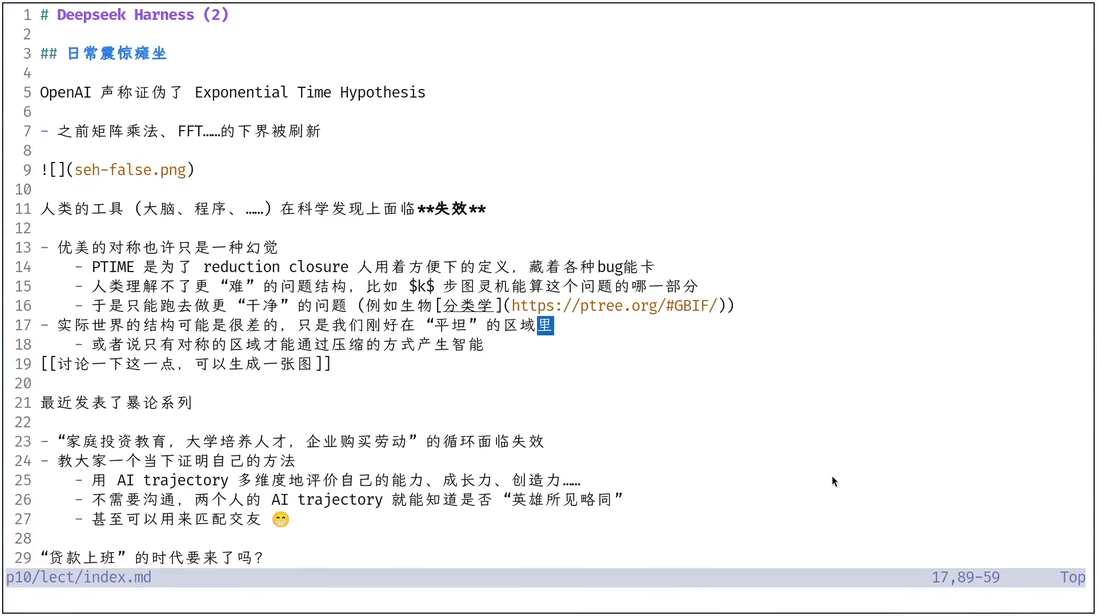
\includegraphics[width=0.92\textwidth]{figures/fig_01_course_outline.png}
\caption{第 10 讲《软件的演化（DeepSeek Harness 2）》课堂大纲视图：涵盖前沿论文讨论、航母百年演化史、软件时间维度与工程品味、以及 DeepSeek Harness 源码提交考古\vtag}
\end{figure}
\srcnote{00:00:00--00:00:15}

\subsection{指数时间假说（ETH）冲击与亚指数精确计数算法}

进入 AI 时代后，计算机科学界几乎每周都在经历“日常震惊综合症”。课堂首先分享了当天早上引发理论计算机科学（TCS）社区震动的一则消息：OpenAI 团队发布预印本论文，声称利用前沿推理模型证伪了统治计算复杂性理论数十年的\textbf{指数时间假说（Exponential Time Hypothesis，简称 ETH）}（图 2）。

\begin{figure}[H]
\centering
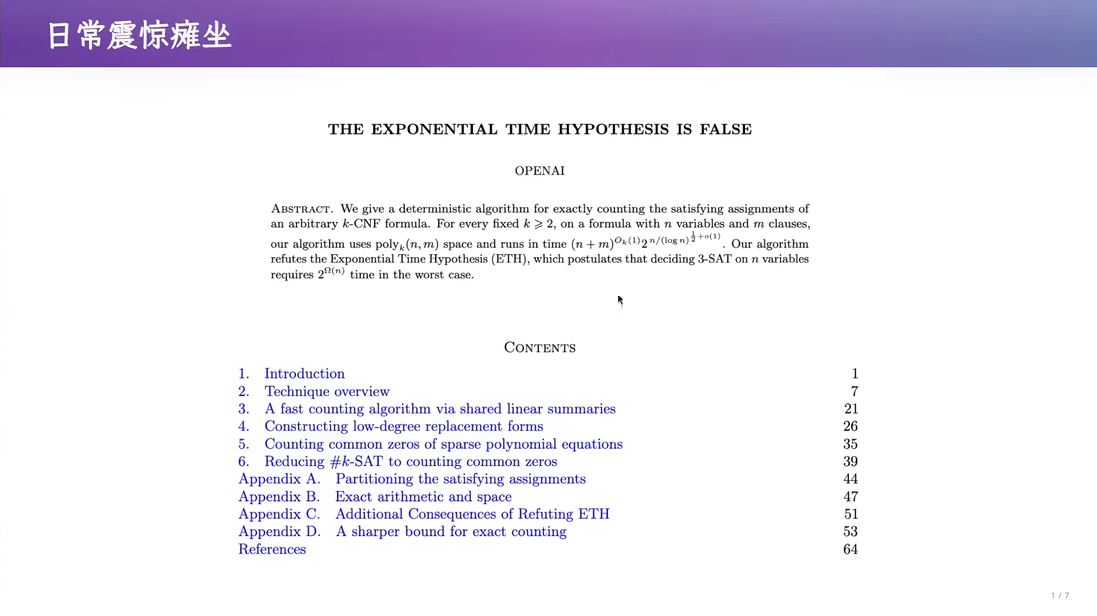
\includegraphics[width=0.92\textwidth]{figures/fig_02_eth_paper.png}
\caption{日常震惊综合症：关于指数时间假说（Exponential Time Hypothesis）被亚指数时间精确计数算法突破的前沿论文摘要与课堂讨论\vtag}
\end{figure}
\srcnote{00:00:30--00:00:45}

所谓指数时间假说（Impagliazzo \& Paturi，1999），比著名的 $\mathrm{P} \neq \mathrm{NP}$ 猜想更为强硬：$\mathrm{P} \neq \mathrm{NP}$ 仅断言 3-SAT 问题不存在多项式时间算法，而 ETH 进一步断言 3-SAT 甚至不存在\textbf{亚指数时间（Sub-exponential Time，$2^{o(n)}$）}算法，即任何确定性算法在最坏情况下的运行时间下界必然形如 $2^{\delta n}$（其中 $\delta > 0$ 为常数）。然而，图 2 展示的论文摘要给出了一个针对任意固定子句宽度 $k \ge 2$ 的 $k$-CNF 公式精确计数（Exact Counting，即 \texttt{\#k-SAT}）确定性算法，其运行时间上界为：

\begin{equation}
T(n, m) = (n + m)^{O_k(1)} \cdot 2^{\frac{n}{(\log n)^{1/2 + o(1)}}}
\end{equation}

其中各符号的物理与数学含义如下：
\begin{itemize}
    \item $T(n, m)$：确定性算法统计满足赋值的精确数量（Exact Number of Satisfying Assignments）所需的最坏运行时间步数；
    \item $n$：输入的合取范式（$k$-CNF）布尔公式中包含的布尔变量总数；
    \item $m$：输入的 $k$-CNF 公式中包含的子句（Clauses）总数，每个子句至多包含 $k$ 个文字（Literals）；
    \item $O_k(1)$：仅依赖于固定子句宽度 $k$ 的常数指数项，管理多项式级的预处理与递归树开销；
    \item $(\log n)^{1/2 + o(1)}$：出现在指数分母上的对数根号修正因子；正是由于分母随着 $n \to \infty$ 趋于无穷大，指数部分 $\frac{n}{(\log n)^{1/2 + o(1)}} = o(n)$ 严格小于线性阶，从而在渐近意义上打破了 $2^{\Omega(n)}$ 的指数壁垒。
\end{itemize}

\subsection{人类数学工具的边界：为什么 \texttt{PTIME} 是一种“函数复合幻觉”？}

这则理论突破引发了一个更深层的科学哲学追问：\textbf{为什么人类数学家研究了半个世纪都默认 3-SAT 需要 $2^{\Omega(n)}$ 时间，甚至把整个细粒度复杂性理论（Fine-Grained Complexity）建立在 ETH 之上？}蒋老师在幻灯片中指出，这暴露了人类认知工具（人脑与传统符号推演）的固有边界（图 3）。

\begin{figure}[H]
\centering
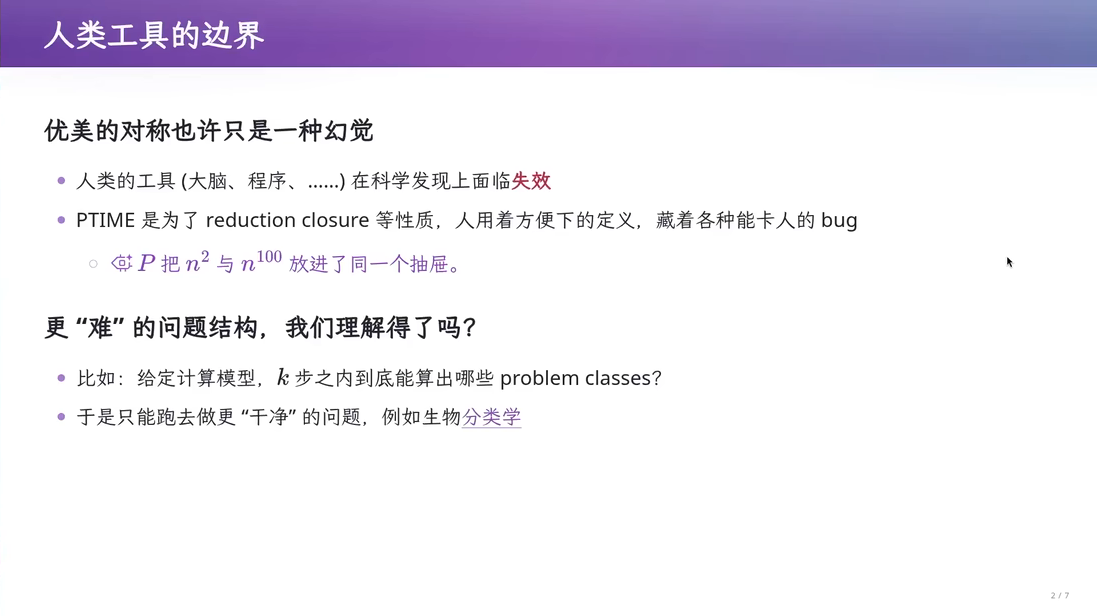
\includegraphics[width=0.92\textwidth]{figures/fig_03_human_tool_limits.png}
\caption{人类工具的边界：多项式时间（\texttt{PTIME}）满足归约与函数复合闭包的人为构造，对比给定形式化 RAM 模型运行 $K$ 步的真实计算图景\vtag}
\end{figure}
\srcnote{00:01:15--00:01:30}

在本科《计算理论》或《算法设计与分析》教材中，我们总是把多项式时间复杂性类 $\mathrm{P}$（即 $\mathrm{PTIME} = \bigcup_{c \ge 1} \mathrm{TIME}(n^c)$）视为“可高效求解（Tractable）”的同义词。但仔细审视这一定义就会发现其荒谬之处：一个运行时间为 $n^2$ 的算法在工业界切实可用，而一个运行时间为 $n$ 的 100次方（$n^{100}$）的算法，哪怕当输入规模 $n = 2$ 时，其计算步数 $2^{100} \approx 1.26 \times 10^{30}$ 也早已超过宇宙年龄内的总原子振动次数！既然 $n^{100}$ 在物理世界中比 $2^{\sqrt{n}}$ 慢得多，为什么理论计算机科学家非要把 $n^2$ 和 $n$ 的 100次方塞进同一个名为 $\mathrm{PTIME}$ 的抽屉里？

答案只有一个：\textbf{为了凑出归约（Reduction）与函数复合的代数闭包性质（Closure under Function Composition）}。当我们将一个规模为 $n$ 的问题实例通过算法 $A_1$（耗时 $p_1(n)$，输出规模至多为 $p_1(n)$）归约给另一个算法 $A_2$（耗时 $p_2(\cdot)$）时，复合算法的总运行时间满足：

\begin{equation}
T_{\mathrm{comp}}(n) = p_1(n) + p_2\bigl(p_1(n)\bigr) = O\bigl(n^{c_1 \cdot c_2}\bigr) \in \mathrm{PTIME}
\end{equation}

其中各符号的含义如下：
\begin{itemize}
    \item $T_{\mathrm{comp}}(n)$：两个多项式时间算法串联复合（或子程序调用）后的总运行时间上界；
    \item $p_1(n) = O(n^{c_1})$：外层归约或预处理算法的时间与输出体积上界，其中 $c_1 \ge 1$ 为常数阶；
    \item $p_2(m) = O(m^{c_2})$：内层目标求解算法在输入规模为 $m = p_1(n)$ 时的运行时间上界，其中 $c_2 \ge 1$ 为常数阶；
    \item $c_1 \cdot c_2$：多项式复合后的新指数阶；无论复合多少次，多项式套多项式依然是多项式（$\mathrm{P} \circ \mathrm{P} = \mathrm{P}$）。
\end{itemize}

\begin{importantbox}{核心洞见：形式化 RAM 模型的 $K$ 步可达集才是真实物理对象}
人类之所以定义 $\mathrm{PTIME}$，并不是因为自然界偏爱多项式，而是因为\textbf{人类大脑只能驾驭具有良好代数闭包性质的数学工具}。在真实的计算机工程中，真正有意义的根本问题是：\textbf{“给定一个形式化的随机存取机（RAM 模型，配备寄存器、ALU 与内存阵列），在严格给定的 $K$ 个时钟周期（$K$ steps）内，究竟能够判定和计算出哪些问题集合？”}遗憾的是，当 $K$ 固定时，这个集合边界极其崎岖、毫无代数对称性可言，完全超出了人类纸笔证明的压缩能力；而拥有超长上下文与大规模算力搜索能力的 AI，恰恰能够深入这些缺乏简洁闭包的“崎岖地带”寻找非直觉的组合结构。
\end{importantbox}

\begin{knowledgebox}{复杂性理论反思：为什么 \texttt{PTIME} 在工程实践中不够用？}
在经典计算复杂性理论中，$\mathrm{PTIME}$ 的设计初衷是获得归约与子程序复合的代数封闭性（$p_1(p_2(n))$ 仍为多项式），从而屏蔽具体机器模型（图灵机单带、多带或 RAM 模型）的底层差异。但在真实系统工程中，内存层次结构（Cache 行大小）、固定时钟预算 $K$ 下的吞吐上界才是硬约束。认识这一差异，能帮助我们跳出“只要渐近复杂度相同就等价”的教条。
\end{knowledgebox}

\subsection{从生物分类树到诺特定理：我们刚好站在“平坦”的地方}

为了进一步阐明“人类科学工具偏爱平滑与对称结构”的现象，蒋老师在课堂上打开了交互式生命之树可视化网站（\texttt{https://ptree.org/\#GBIF/}），展示了地球生物分类学（界、门、纲、目、科、属、种）的庞大演化树，并放大到寒武纪布尔吉斯页岩古生物 \textit{Capinatator praetermissus} 的分类节点（图 4）。

\begin{figure}[H]
\centering
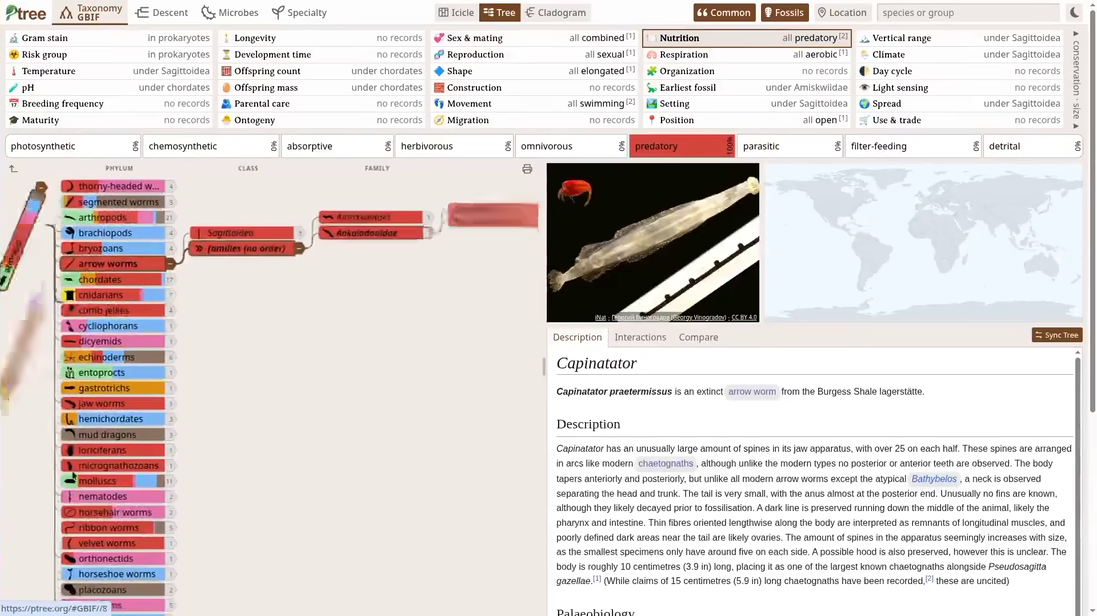
\includegraphics[width=0.92\textwidth]{figures/fig_04_tree_of_life.png}
\caption{生物分类树（Tree of Life）交互可视化：宏观物种呈现清晰的树状分叉，但在微生物水平基因转移与杂交网状演化下退化为复杂的图结构\vtag}
\end{figure}
\srcnote{00:06:45--00:07:00}

在中学与大学生物课本里，我们习惯把物种演化画成一棵干净的树（Tree）。然而，一旦深入到细菌、古菌与病毒等微观生物领域，频繁的\textbf{水平基因转移（Horizontal Gene Transfer，HGT）}与内共生融合就会彻底打破树状单亲继承假设——真实的生命演化史根本不是一棵树，而是一张高度纠缠的\textbf{有向无环图甚至一般图（Graph）}。人类之所以画出“界门纲目科属种”的树，同样是因为树具有极简的递归层次结构，便于人脑记忆与检索。

这引出了本节最具哲学穿透力的命题——\textbf{“我们刚好站在平坦的地方”}（图 5）：

\begin{figure}[H]
\centering
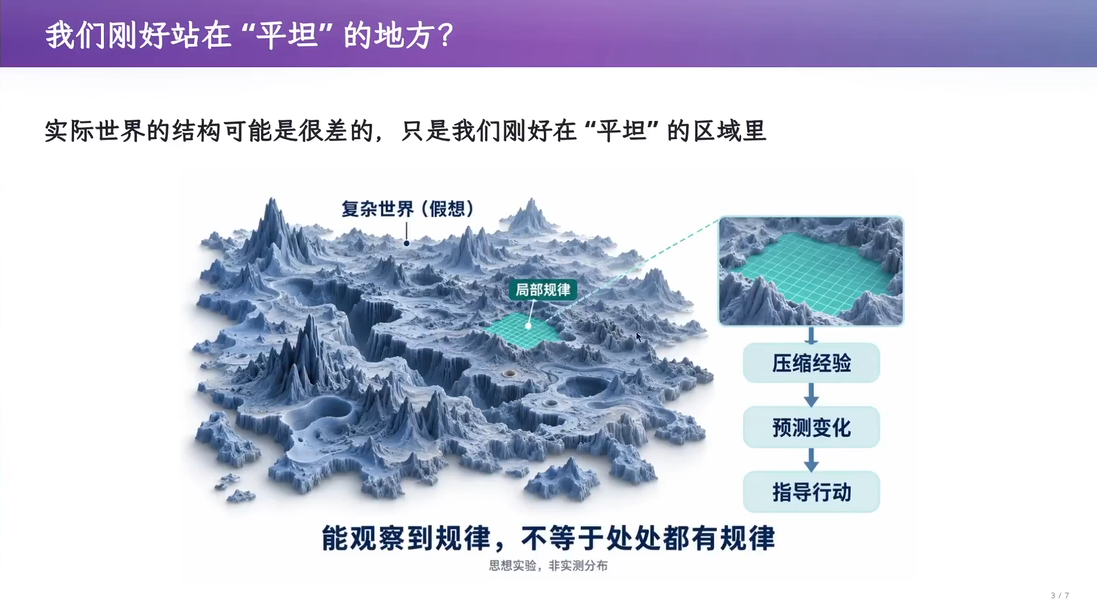
\includegraphics[width=0.92\textwidth]{figures/fig_05_flat_region_symmetry.png}
\caption{我们刚好站在平坦的地方：物理世界的对称性（诺特定理）导出守恒量与可压缩经验规律，但局部存在规律不代表全局处处平坦\vtag}
\end{figure}
\srcnote{00:07:45--00:08:00}

\begin{enumerate}
    \item \textbf{对称性 $\to$ 守恒量 $\to$ 规律可压缩 $\to$ 智能可演化}：根据理论物理学家埃米·诺特（Emmy Noether）于 1918 年证明的\textbf{诺特定理（Noether's Theorem）}，物理系统作用量的每一种连续对称性都严格对应一个守恒定律——时间平移对称性对应\textbf{能量守恒}，空间平移对称性对应\textbf{动量守恒}，空间旋转对称性对应\textbf{角动量守恒}。正因为我们所处的宏观低速物理宇宙具备高度的时空对称性，过去总结的经验在明天依然成立，海量观测数据才能被压缩成寥寥数行的牛顿力学与麦克斯韦方程组，生物大脑与大语言模型的注意力机制（Attention）也才能通过拟合局部梯度学到泛化规律（Scaling Law）。
    \item \textbf{幸存者偏差警示——“能观察到规律，不等于处处都有规律”}：正如微积分利用泰勒展开（$f(x + \Delta x) \approx f(x) + f'(x)\Delta x$）将非线性流形在局部切空间近似为平坦的欧氏空间，人类已有科学体系只覆盖了自然界与数学空间中“可微、对称、可压缩”的平坦绿洲。在自动机理论、形式化验证与复杂软件系统的全局状态空间中，大量区域本质上是不可压缩、充满组合爆炸与不连续相变的荒原。
\end{enumerate}

\subsection{本章小结}

本章从 OpenAI 挑战指数时间假说（ETH）的亚指数精确计数算法切入，剖析了人类科学认知的底层机理：无论是理论计算机科学中的 $\mathrm{PTIME}$ 闭包，还是生物学中的生命分类树，抑或物理学中的对称守恒律，本质上都是人类在“平坦区域”建立的理想化模型。理解这一边界，有助于我们在面对复杂软件系统与 AI 智能体时，放弃寻找“一招鲜的万能闭式公式”，转而正视演化过程中的具体工程约束与历史路径依赖。

% =========================================================================
% SECTION 2
% =========================================================================
\section{教育循环松动与 AI Trajectory 简历革命}

从科学认知的边界回到每位同学切身相关的现实问题：在 AI 编程智能体（Coding Agent）能力狂飙突进的 2026年，计算机专业本科生与研究生的教育投资回报率正在发生怎样的结构性剧变？

\subsection{教育闭环的松动与 Spence 信号理论失灵}

在过去四十年的信息化浪潮中，高等教育一直运转在一个极其稳固的正反馈闭环之上（图 6）：
\begin{itemize}
    \item \textbf{家庭投资}：父母与学生投入四年至七年的学费、生活费与青春时间（机会成本）；
    \item \textbf{大学培养与筛选}：高校通过高考录取、课程考试、GPA 排名与毕业设计，对学生进行知识传授与能力背书；
    \item \textbf{企业购买与初级岗培养}：科技企业招聘应届毕业生（Junior Engineer），容忍其入职前 6 至 12 个月的低产出期，由资深工程师（Senior Engineer）通过 Code Review 与师徒制（Mentorship）将其培养成下一代骨干，企业再以高薪回报兑现家庭的教育投资。
\end{itemize}

\begin{figure}[H]
\centering
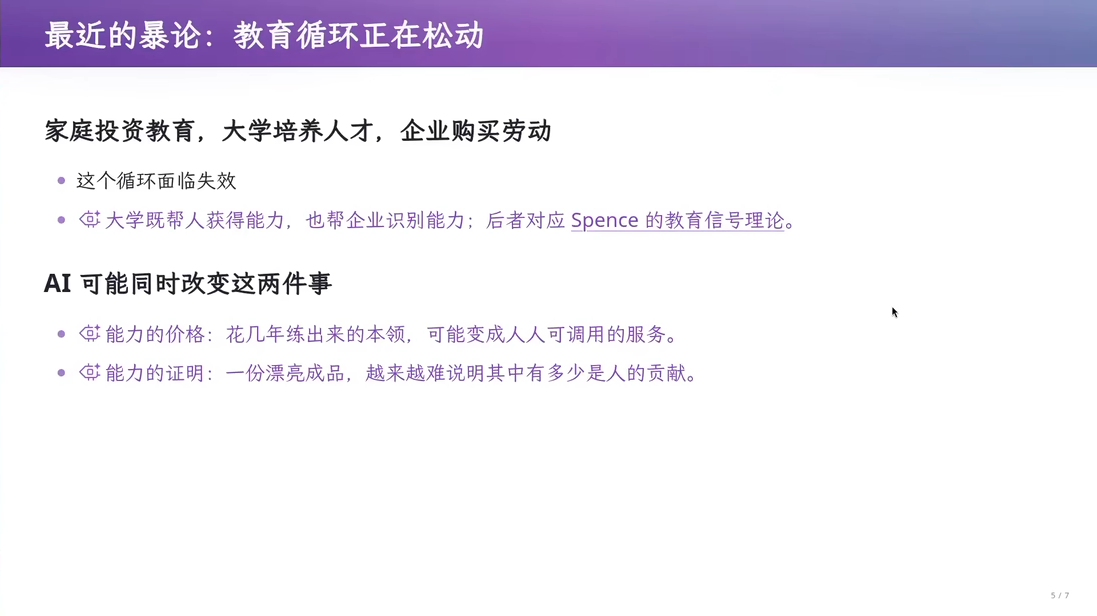
\includegraphics[width=0.92\textwidth]{figures/fig_06_education_loop_spence.png}
\caption{教育循环正在松动：当 \texttt{Senior + Agent > Junior} 时企业招聘应届生动力下降，同时 Spence（1973）教育信号机制因人机成果混同而面临失真\vtag}
\end{figure}
\srcnote{00:09:00--00:09:15}

然而，这一延续数十年的闭环正在两个关键节点上同时发生断裂：
\begin{enumerate}
    \item \textbf{生产力不等式的反转（\texttt{Senior + Agent > Junior}）}：过去资深工程师必须把繁琐的样板代码、单元测试编写、日志排查分包给应届生；而今天，一位架构清晰、懂得拆解问题的 Senior 配合十几个并发运转的 Claude Code / DeepSeek Harness 智能体，其吞吐量远超带领五名初级工程师，且无需承担沟通摩擦与返工成本。这导致硅谷与国内大厂初级岗位（Headcount）急剧收缩。
    \item \textbf{Spence（1973）劳动力市场信号理论（Job Market Signaling）的失灵}：诺贝尔经济学奖得主迈克尔·斯宾塞（Michael Spence）在 1973 年指出，文凭与课程大作业之所以能充当有效信号，前提是\textbf{“低能力者伪造该信号的边际成本显著高于高能力者”}。但在生成式 AI 时代，无论是满分的课程实验大作业、精美的个人博客，还是 GitHub 上一个看似完备的开源项目，面试官拿到一份静态成品时，已经\textbf{无法区分其中哪部分来自候选人的真实思考，哪部分来自 AI 的一键生成}。
\end{enumerate}

\begin{knowledgebox}{经济学视角：Spence（1973）信号博弈模型与筛选成本反转}
在斯宾塞信号模型中，当且仅当高能力者发送信号 $s$ 的成本 $c(s, \theta_H)$ 显著低于低能力者 $c(s, \theta_L)$ 时，市场才存在分离均衡（Separating Equilibrium）。生成式 AI 将制造静态代码产物的成本 $c(s_{\mathrm{artifact}}, \theta_L)$ 压缩至趋近于零，导致静态简历陷入混同均衡（Pooling Equilibrium）；而长周期的 \texttt{AI Trajectory} 因包含数千次实时决策与抽样问答校验，重新恢复了极高的伪造壁垒。
\end{knowledgebox}

\subsection{用 AI Trajectory 证明自己：不可伪造的过程轨迹简历}

既然静态的“结果产物（Artifact）”已经丧失了区分度，年轻工程师靠什么向未来的团队证明自己具有极高的培养价值？蒋老师给出了一个极具前瞻性的方案——\textbf{用你与 AI 协同工作的完整过程轨迹（AI Trajectory）作为新世代简历}（图 7）。

\begin{figure}[H]
\centering
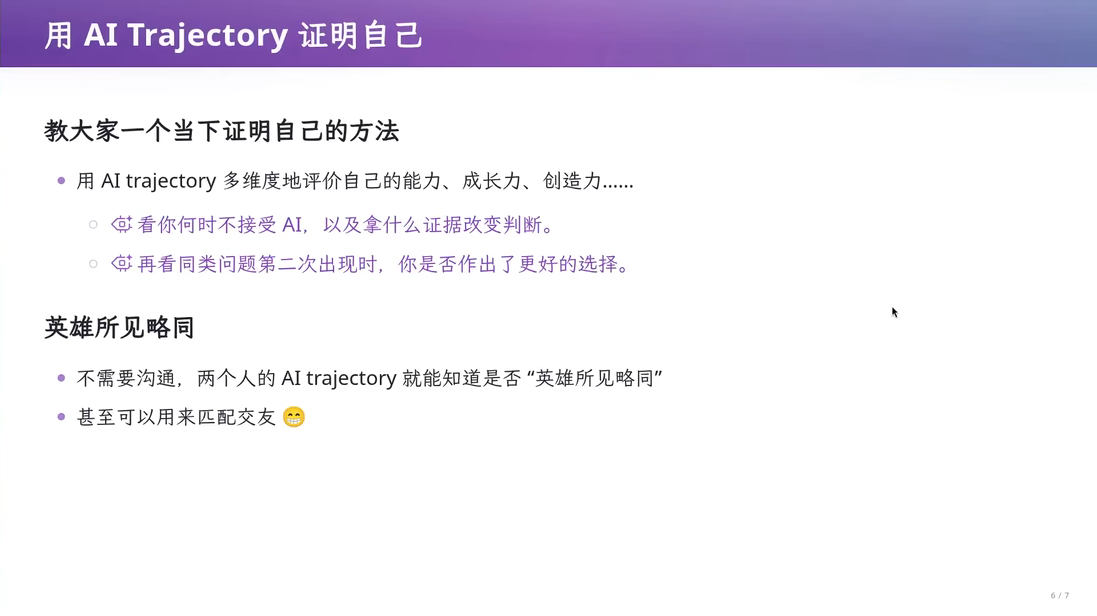
\includegraphics[width=0.92\textwidth]{figures/fig_07_ai_trajectory_resume.png}
\caption{用 AI Trajectory 证明自己：通过不可伪造的高密度人机交互事实日志，展示何时拒绝 AI、凭何证据推翻判断，并支持面试随机采样核验与双人 Trajectory 共识碰撞\vtag}
\end{figure}
\srcnote{00:10:30--00:10:45}

为什么一份长达数月、包含数千次交互的 \texttt{AI Trajectory}（如 \texttt{~/.pi/agent/} 或 Claude / Cursor 本地会话日志库）能够重建信任？课堂结合黑板板书（图 8）剖析了三大核心机制：

\begin{figure}[H]
\centering
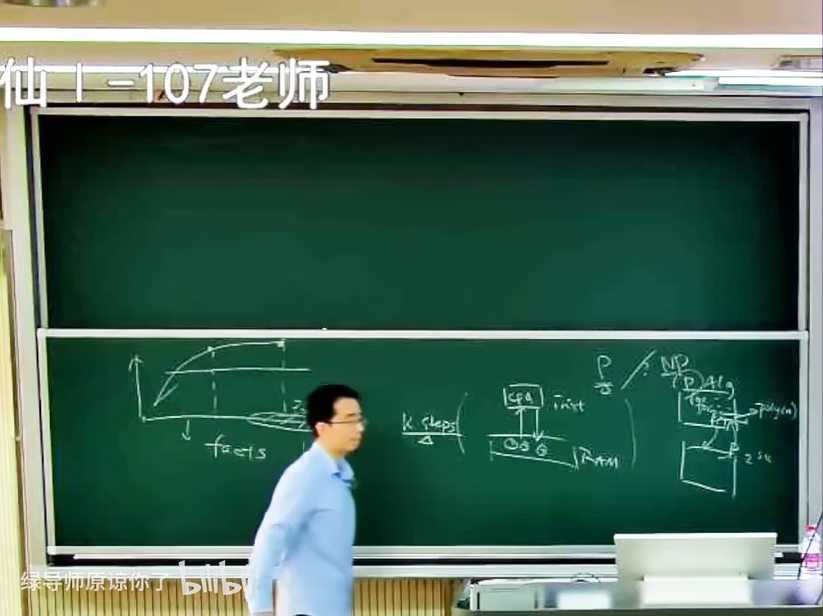
\includegraphics[width=0.82\textwidth]{figures/fig_08_board_growth_curves.png}
\caption{课堂板书解析：左侧描绘两位高考同分学生在大学四年中的真实潜力演化曲线分化（突破阈值 vs 停滞），右侧示意多维能力向量评估\vtag}
\end{figure}
\srcnote{00:13:30--00:13:45}

\begin{enumerate}
    \item \textbf{过程信号的三个黄金观测点}：
    \begin{itemize}
        \item \textbf{你什么时候不接受 AI 的输出？}平庸的使用者只会无脑复制粘贴或复读报错信息“它还是挂了，请修好”；而优秀的工程师会在 AI 生成出看似能跑但破坏模块边界的代码时立刻喊停（\texttt{Operation aborted}），指出其架构隐患。
        \item \textbf{你拿什么证据改变自己的判断？}当系统出现诡异 Bug 时，你是靠猜测试探，还是构造最小可复现用例（MRE）、二分排查日志、设计可证伪的实验来收敛假设空间？
        \item \textbf{同一个问题第二次出现时，你的选择有没有更好？}图 8 黑板左侧画出了两条从同一高考分数起点出发的成长曲线：真正高潜力的学生在遇到挫折后会把教训沉淀为工具脚本或个人 Skill，使其能力曲线突破平坦期实现非线性跃升。
    \end{itemize}
    \item \textbf{密码学级别的防伪校验（随机抽样面试法）}：有人也许会问：“AI Trajectory 难道不能让 AI 伪造一份吗？”蒋老师指出，数千万 Token 的日常试错、时间线交叉引用与思维演进具有极高的信息熵。面试官根本不需要读完所有日志，只需在面试现场随机抽样：\textbf{“我看你在 2026年 3 月 10 日下午花三个小时重构了状态同步模块，当时为什么否决了第二种方案？”}如果是本人亲历的痛苦调试，细节必然脱口而出；如果是伪造的日志，哪怕当场搜索也无法在十秒内还原当时的上下文权衡。
    \item \textbf{Agent 读 Trajectory 实现“英雄所见略同”的双向匹配}：当两位开发者都拥有半年以上的高质量 AI Trajectory 时，双方的 Agent 可以直接交换阅读对方的非涉密工程轨迹，自动找出两人在技术审美、代码洁癖与架构取舍上的共鸣点——这不仅是招聘面试的终极形态，甚至能成为寻找创业合伙人、学术合作者乃至知己好友的全新基础设施。
\end{enumerate}

\subsection{上学作为“期货投资”与“贷款上班”的极权推演}

在这一章的尾声，蒋老师用经济学视角审视了高等教育的本质（图 9）：\textbf{上学本身就是一笔高杠杆的“人力资本期货投资”}。学生在入学选专业时买入看涨期权，投入四年时间和学费，押注四年后毕业时就业市场对该技能的现货定价；然而没有任何一家企业在录取通知书上签署远期回购协议。

\begin{figure}[H]
\centering

\includegraphics[width=0.92\textwidth]{figures/fig_09_school_futures_loan.png}
\caption{上学是一笔面向未来的期货投资：关于人力资本加速折旧、“交保证金贷款上班”的极端思想实验与 AI 能力核不扩散思考\vtag}
\end{figure}
\srcnote{00:17:30--00:17:45}

\begin{warningbox}{思想实验警示：警惕技能折旧周期短于学习周期}
沿着“初级工程师培养成本高于 AI 替代成本”的逻辑推演，课堂开了一个发人深省的黑色幽默玩笑——\textbf{“贷款上班”}：未来某天企业会不会要求应届生先交一笔保证金或自费购买在岗训练算力，若三个月内证明自己比 AI 强则留下返还，否则没收保证金？这一极端暴论背后是一个严肃的社会学与工程学命题：当 AI 让单项编码技能的半衰期缩短到以月计算时，死背某个框架 API 的“现货型学生”必然面临技能迅速贬值；唯有掌握\textbf{系统演化规律、审美判断（Taste）与驾驭智能体群（Harness）}的底层能力，才能在剧烈波动的技术期货市场中立于不败之地。
\end{warningbox}

\subsection{本章小结}

本章剖析了 AI 时代“家庭—大学—企业”教育循环松动的深层经济学原因，指出静态作业与项目成品已因 Spence 信号失灵而难以自证能力。破局之道在于从今天起有意识地积累并打磨自己的 \textbf{AI Trajectory}，在每一次与 AI 的博弈中留下“有理有据的拒绝、科学严谨的取证、持续进化的抽象”三类高价值工程痕迹。

% =========================================================================
% SECTION 3
% =========================================================================
\section{航母是怎么造出来的：从风帆、明轮汽船到中途岛号的百年演化}

在回顾上一讲《DeepSeek Harness (1)》的反馈时，蒋老师指出（图 10）：如果把各类大语言模型（Claude、DeepSeek、GPT）比作早期的双翼螺旋桨飞机，那么 \texttt{DeepSeek Harness (dsh)} 就像是一艘\textbf{航空母舰（Aircraft Carrier）}——它本身不直接去轰炸目标，而是为无数尚处于快速迭代试验阶段的智能体提供统一的甲板调度、弹药补给（Context 管理）、安全阻拦索（Guardrails）与机库维护（Session 持久化）。正如 1922年的美国海军第一艘航母兰利号（USS Langley）作为舰载航空的试验平台，哪怕它自己后来退居二线，它摸索出的起降调度范式也完整传承给了后世的所有现代航母。

\begin{figure}[H]
\centering
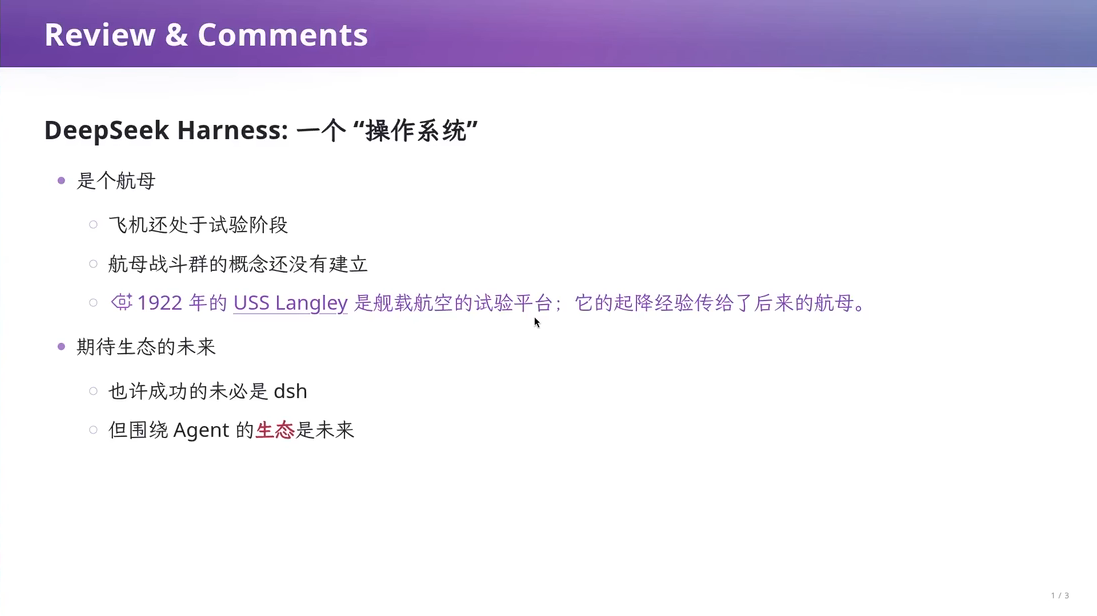
\includegraphics[width=0.92\textwidth]{figures/fig_10_review_dsh_os.png}
\caption{上讲回顾与延伸：DeepSeek Harness 作为承载智能体起降的“航母级操作系统”，以及 1922年兰利号（USS Langley）试验平台的历史隐喻\vtag}
\end{figure}
\srcnote{00:19:45--00:20:00}

\subsection{圣地亚哥的工程震撼：1945年的中途岛号（USS Midway）}

这就引出了一个令人着迷的工程史问题：\textbf{像航空母舰这样包含数百万个零件、数千公里管线、两千余名船员协同运转的超级复杂系统，究竟是如何在没有现代计算机辅助设计（CAD）的 1945年被人类造出来的？}

2019年，蒋老师在加州圣地亚哥港实地参观了著名的\textbf{中途岛号航空母舰博物馆（USS Midway，舷号 CV-41）}，并拍下了图 11 的照片。中途岛号于 1945年 9 月下水服役（恰逢第二次世界大战结束之后），在 1970年代经历了大规模现代化改装，直到 1992年还在海湾战争“沙漠风暴”行动中担任美军波斯湾航空母舰战斗群旗舰，服役近半个世纪后退役成为博物馆。

\begin{figure}[H]
\centering
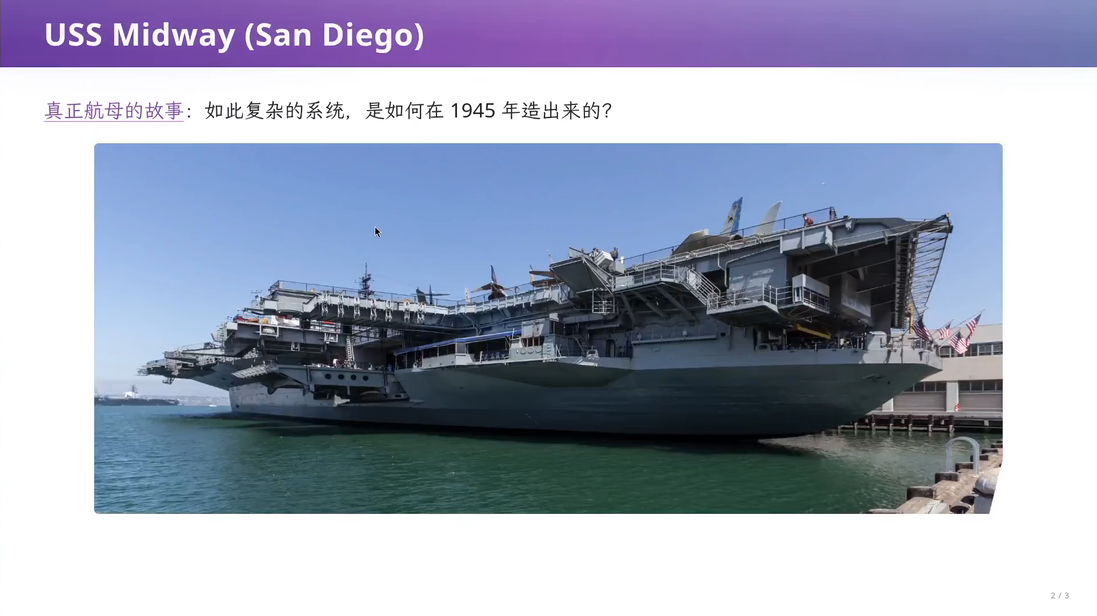
\includegraphics[width=0.92\textwidth]{figures/fig_11_uss_midway_photo.png}
\caption{圣地亚哥中途岛号航空母舰（USS Midway，CV-41，主讲教师 2019年实拍）：如此庞大的复杂工程系统是如何在 1945年造出来的？\vtag}
\end{figure}
\srcnote{00:23:45--00:24:00}

走进 Midway 幽深狭窄的甲板下层舱室，最直观的震撼来自于头顶与四周密如蛛网的高压蒸汽管道、电力电缆、声力电话网与损管（Damage Control）阀门（图 12）。博物馆里的讲解员大多是当年在 Midway 上服役过的美国海军老兵。当被问及“你们当年在船上是怎么理解这套如此复杂的系统的？”时，老兵的回答道破了大型系统工程的真谛：

\begin{knowledgebox}{航母老兵的工程法则：操作手册（Operating Manual）与状态机解耦}
在航空母舰上服役的水兵与军官，\textbf{没有任何一个人需要（也不可能）在脑子里装下整艘航母的全局图纸}。每个舱室、每个战位都有一本千锤百炼的\textbf{《标准操作手册》（Standard Operating Manual）}：当仪表盘指针越过红线、或者损管警报响起时，轮机部门（M Division）的水兵只需严格按照手册第几页第几条转动指定编号的阀轮、完成局部状态交接。整艘航母之所以能作为一个有机整体在战火中高速运转，靠的正是\textbf{清晰的职责分工、标准化的接口交接与确定性的局部状态机规程}。
\end{knowledgebox}

\begin{figure}[H]
\centering
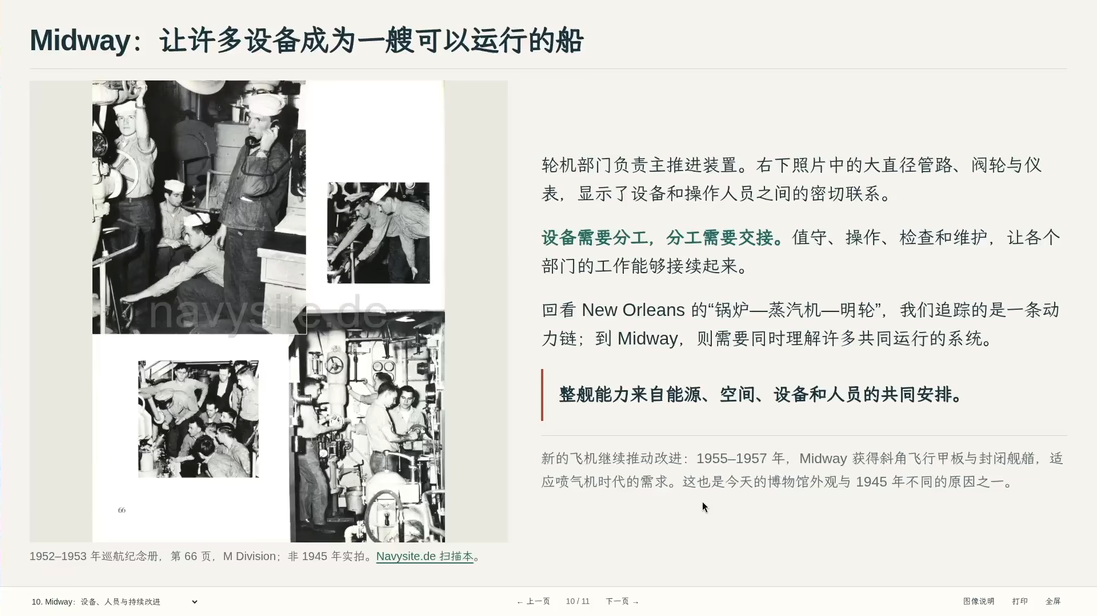
\includegraphics[width=0.92\textwidth]{figures/fig_12_midway_internal_manual.png}
\caption{Midway 内部轮机部门（M Division，1952--1953 年巡航纪念册）与 1955--1957 年斜角甲板改装：设备需要分工，分工需要交接，整舰能力来自能源、空间、设备与人员的共同安排\vtag}
\end{figure}
\srcnote{00:25:00--00:25:15}

\clearpage
\subsection{从风帆到海上机场：四代舰船的平滑状态转移}

为了看清 1945年的 Midway 是如何从简单船只一步步长出来的，蒋老师制作了一份专门的交互式历史考证讲义《从风帆到海上机场》（图 13），选取了跨越四个半世纪的四艘标志性舰船，还原了每次只往前迈出一个小增量（$+\Delta$）的演化轨迹：

\begin{figure}[H]
\centering
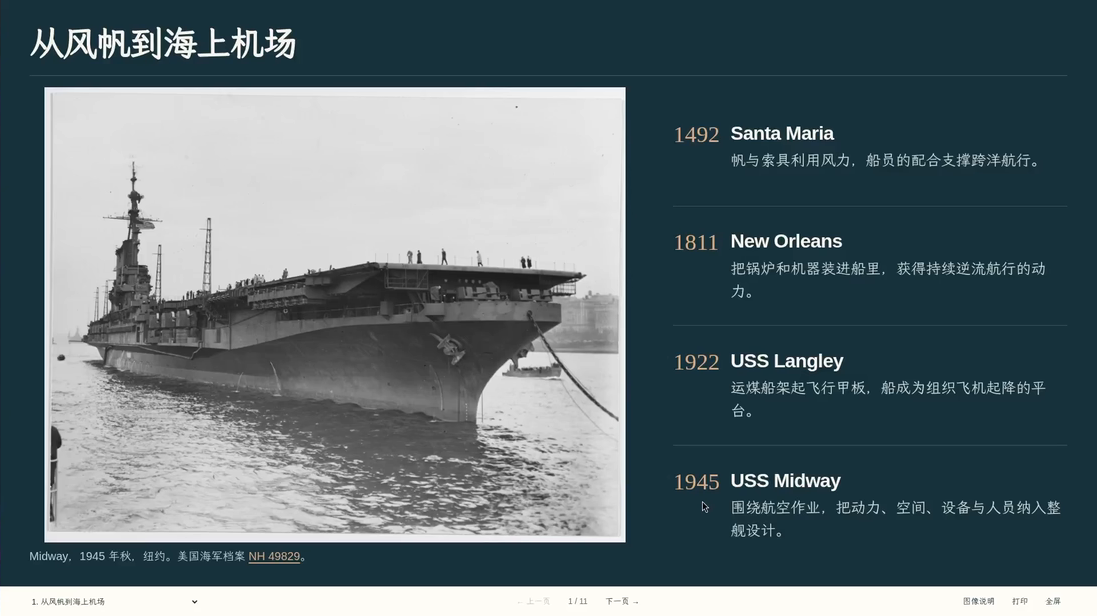
\includegraphics[width=0.92\textwidth]{figures/fig_13_four_ships_overview.png}
\caption{从风帆到海上机场的四代舰船演化总览：1492年 Santa Maria、1811年 New Orleans、1922年 USS Langley 与 1945年 USS Midway\vtag}
\end{figure}
\srcnote{00:27:30--00:27:45}

\subsubsection{第一代（1492年）：Santa Maria——用帆与索具驾驭船外风力}

1492年，哥伦布率船队首次横渡大西洋抵达加勒比海（原船于 1492年圣诞节在 Hispaniola 附近搁浅，图 14 为巴塞罗那海事博物馆制作、Smithsonian 馆藏的 1965 年考证复原模型）。在圣玛丽亚号（Santa Maria）上，\textbf{动力完全来自船外的自然风力}，船上没有任何动力机器；船员通过调整横帆、三角帆的姿态与繁复的索具（Rigging），将变幻莫测的风力转化为推进力，并通过桅杆与船体肋骨传递受力。此时整船的机械复杂度完全处于单个人类工匠（造船木匠与船长）可以直观理解的范围内。

\begin{figure}[H]
\centering

\includegraphics[width=0.92\textwidth]{figures/fig_14_1492_santa_maria.png}
\caption{1492年圣玛丽亚号（Santa Maria）：风提供动力，帆与索具提供控制；动力来自船外，受天气、航海经验与物资储备共同约束\vtag}
\end{figure}
\srcnote{00:28:15--00:28:30}

\subsubsection{第二代（1811年--1812年）：New Orleans——把蒸汽动力链装进船里}

帆船最大的痛点是无法在内河逆流而上或无风航行。到了 1811年，由蒸汽船先驱罗伯特·富尔顿（Robert Fulton）设计、罗伯特·利文斯顿（Robert Livingston）出资、尼古拉斯·罗斯福（Nicholas Roosevelt）参与建造并负责首航的\textbf{新奥尔良号（New Orleans）}在匹兹堡建成（图 15）。它沿俄亥俄河、密西西比河顺流而下，于 1812年成功抵达新奥尔良，并在新奥尔良与 Natchez 之间开展定期内河往返运输。

\begin{figure}[H]
\centering
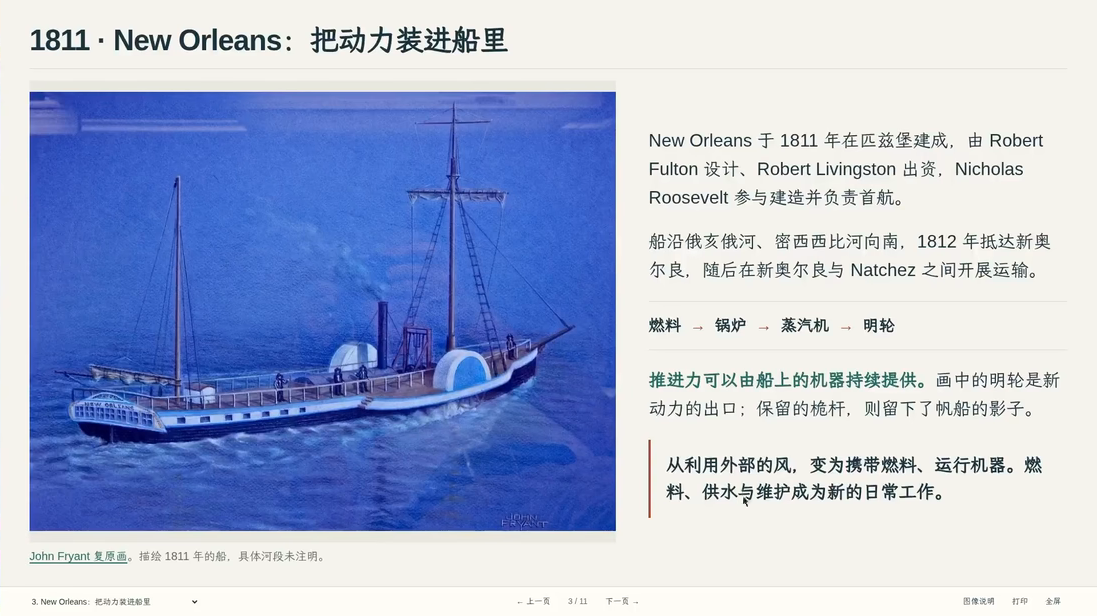
\includegraphics[width=0.92\textwidth]{figures/fig_15_1811_new_orleans.png}
\caption{1811年新奥尔良号（New Orleans，1812年抵达新奥尔良）：把锅炉与蒸汽机装进船里驱动明轮，形成“燃料 $\to$ 锅炉 $\to$ 蒸汽机 $\to$ 明轮”内部动力链\vtag}
\end{figure}
\srcnote{00:29:15--00:29:30}

观察图 15 可以发现两个极有趣的演化细节：
\begin{itemize}
    \item \textbf{为什么中文把现代钢铁巨轮称为“轮船”？}早期的蒸汽船还没有发明高效的船尾水下螺旋桨，而是像水车一样在船体两侧（或船尾）安装巨大的\textbf{明轮（Paddle Wheel）}拍水推进——船体侧面真的装有两个大轮子，“轮船”一词由此得名并沿用至今。
    \item \textbf{保留桅杆的“向后兼容”设计}：仔细看 New Orleans 的复原画，船体中央雖然竖起了冒黑烟的蒸汽锅炉烟囱与蓝色明轮罩，但船头和船尾依然保留了两根高耸的帆船桅杆！这是因为早期蒸汽机故障率高且燃料消耗快，保留风帆作为冗余备份（Fallback）是工程演化过渡期的典型特征。同时，把动力装进船里后，\textbf{“燃料补给、锅炉供水与机器维护”}第一次成为了船员必须面对的日常系统工程。
\end{itemize}

\begin{importantbox}{演化工程学启示：为什么“保留桅杆的明轮船”不是坏设计？}
许多有代码洁癖的工程师在重构时喜欢“一次性彻底重写”，对过渡期的兼容层深恶痛绝。然而 1811年新奥尔良号在安装蒸汽机与明轮的同时保留风帆桅杆，恰恰展示了成熟工程演化的智慧：在新型动力链尚未经过长航程可靠性验证前，保留旧机制作为降级备份（Fallback），是控制单步状态转移风险的核心手段。
\end{importantbox}

\subsubsection{第三代（1913年--1922年）：USS Jupiter $\to$ USS Langley——运煤船长出了飞行甲板}

进入 20 世纪初，莱特兄弟发明飞机后不久，海军开始思考“能否让飞机从船上起飞和降落”。美国海军的第一艘航空母舰\textbf{兰利号（USS Langley，CV-1）}并不是从零画图纸造出来的，而是由一艘 1913年服役的电动推进运煤船\textbf{朱庇特号（USS Jupiter，AC-3）}在 1920 至 1922年改装而成的（图 16）！

\begin{figure}[H]
\centering
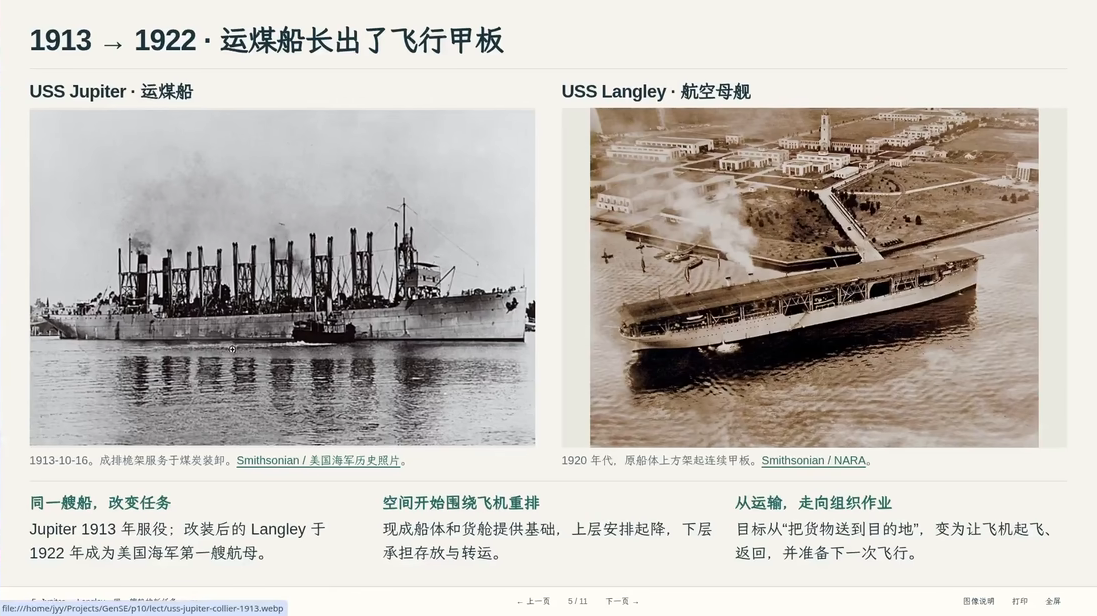
\includegraphics[width=0.92\textwidth]{figures/fig_16_1922_langley_collier.png}
\caption{1913年至 1922年从运煤船 USS Jupiter（左，1913-10-16 拍摄）到美国海军第一艘航空母舰 USS Langley（右，CV-1）：拆掉运煤桁架、在原船体上方架起连续木质飞行甲板\vtag}
\end{figure}
\srcnote{00:31:45--00:32:00}

为什么选运煤船改装航母？因为运煤船原本就有两个天然优势：第一，它的船体下方拥有极其宽敞深邃的\textbf{煤舱（Coal Holds）}，正好可以腾空用来存放拆装或整备状态的双翼机（成为最早的\textbf{机库 Hangar} 雏形）；第二，它原本在甲板上方有一整排用于装卸煤炭的钢铁桁架立柱（图 16 左图），工程师只需把抓斗吊臂拆掉，直接在成排钢柱顶端铺上一层平坦的木板，就用最小的工程改动（Minimum Viable Delta）造出了人类历史上第一块贯通式飞行甲板（图 16 右图）！

然而，在旧架构上“打补丁”必然会暴露出接口衔接的摩擦。图 17 展示了 1923 年 7 月 10 日在兰利号内部拍摄的一张珍贵历史照片：

\begin{figure}[H]
\centering
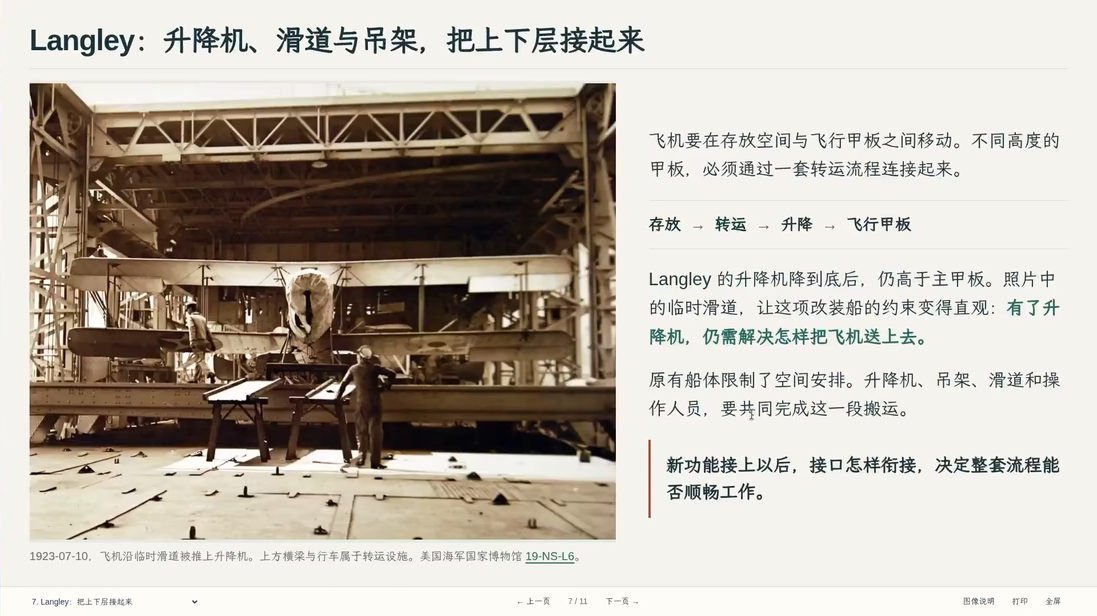
\includegraphics[width=0.92\textwidth]{figures/fig_17_langley_elevator_hangar.png}
\caption{兰利号（USS Langley）内部接口衔接：飞机沿临时滑道被推上升降机，揭示了“存放 $\to$ 转运 $\to$ 升降 $\to$ 飞行甲板”流程中旧船体空间对新功能的约束\vtag}
\end{figure}
\srcnote{00:33:45--00:34:00}

为了把存放在下层煤舱里的飞机送到顶层飞行甲板，兰利号加装了上方横梁行车（吊架）与一部居中升降机（Elevator）。但受限于原有运煤船的船体结构，\textbf{升降机哪怕降到最底部，其平台仍然比主甲板高出一截}！水兵们不得不搭设两块倾斜的木质\textbf{临时滑道（Ramp）}，靠人力把飞机推上升降机平台，再升空送往飞行甲板。这张照片生动诠释了软件与系统演化的一条铁律：\textbf{当你在一个并非为此设计的旧底座上嫁接新功能时，模块之间的胶水层（Glue Code / 临时滑道）往往最能暴露原有架构的边界约束}。

\subsubsection{第四代（1945年）：USS Midway——围绕航空作业从头整舰设计}

兰利号虽然简陋且航速缓慢，但它成功跑通了“海上起降、阻拦索回收、机库转运”的最小闭环。经过列克星敦级、约克城级与埃塞克斯级在太平洋海战中的残酷实战检验，到了 1945年 9 月 10 日服役的\textbf{中途岛号（USS Midway）}，工程师终于不再是在货船上“搭棚子”，而是\textbf{围绕大规模高强度航空作业从头设计整艘巨舰}（图 18、图 19）。

\begin{figure}[H]
\centering
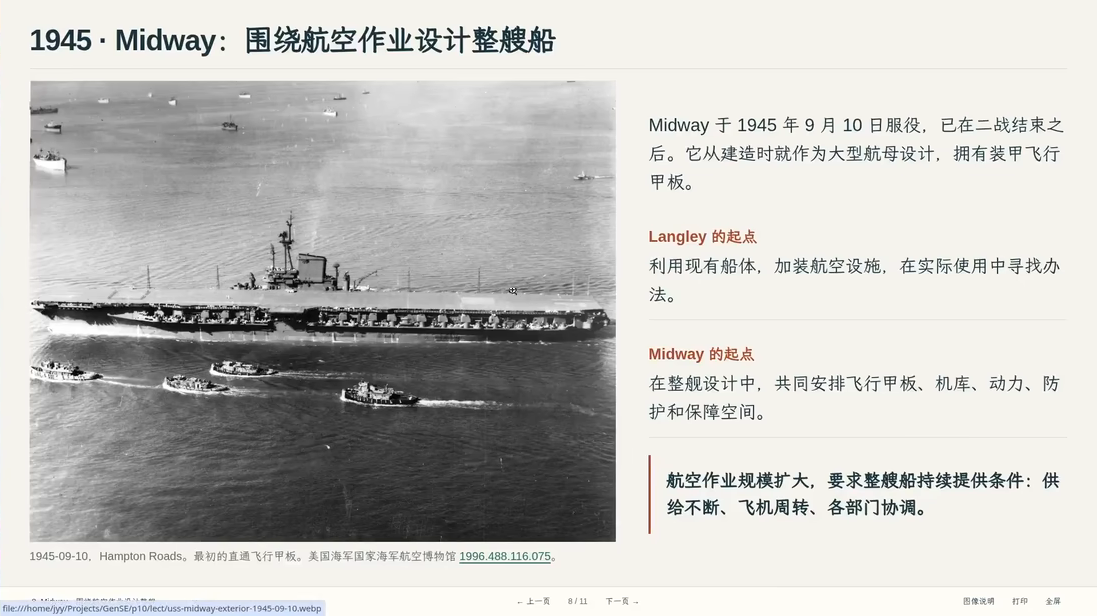
\includegraphics[width=0.92\textwidth]{figures/fig_18_1945_midway_deck.png}
\caption{1945年中途岛号（USS Midway，1945-09-10 摄于 Hampton Roads）：从建造时即作为大型航母整舰设计，拥有装甲飞行甲板，统筹安排甲板、机库、动力、防护与保障空间\vtag}
\end{figure}
\srcnote{00:34:15--00:34:30}

\begin{figure}[H]
\centering
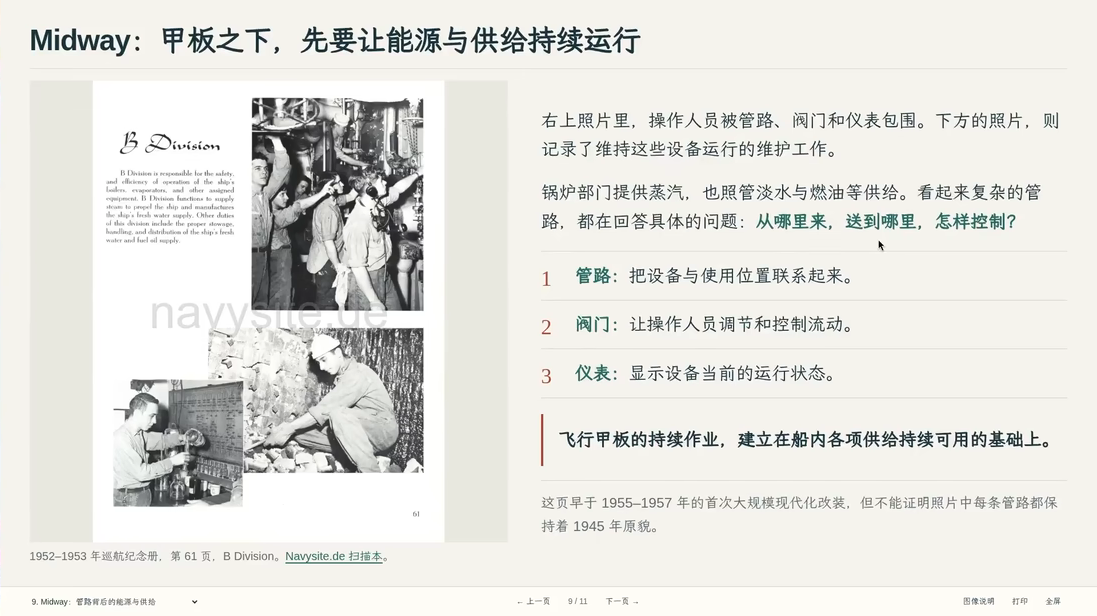
\includegraphics[width=0.92\textwidth]{figures/fig_19_midway_below_deck.png}
\caption{Midway 甲板之下（B Division 锅炉部门，1952--1953 年巡航纪念册第 61 页）：管路、阀门与仪表共同回答“从哪里来、送到哪里、怎样控制”，支撑飞行甲板持续作业\vtag}
\end{figure}
\srcnote{00:34:45--00:35:00}

如图 19 所示，在 Midway 的装甲飞行甲板之下，锅炉部门（B Division）的每一根管路（连接设备与使用位置）、每一个阀门（调节与控制流动）和每一块仪表（显示当前运行状态）都在回答三个确定性的系统问题：\textbf{“能量与物质从哪里来？送到哪里去？怎样安全控制？”}到了 1955--1957 年喷气式舰载机时代来临，Midway 又在此底座上完成了斜角飞行甲板（Angled Flight Deck）与封闭式飓风舰艏的现代化改装，使起飞与降落作业得以同时安全进行。

\subsection{四代舰船演化对比与 AI 时代的“大跨步探路 + 回退重构”范式}

图 20 与表 1 系统总结了从 1492年到 1945年四代舰船的技术能力跃迁规律：\textbf{每当系统增加一种核心外部能力，就必须重新安排内部的能量流、空间流与人员协同关系}。

\begin{figure}[H]
\centering
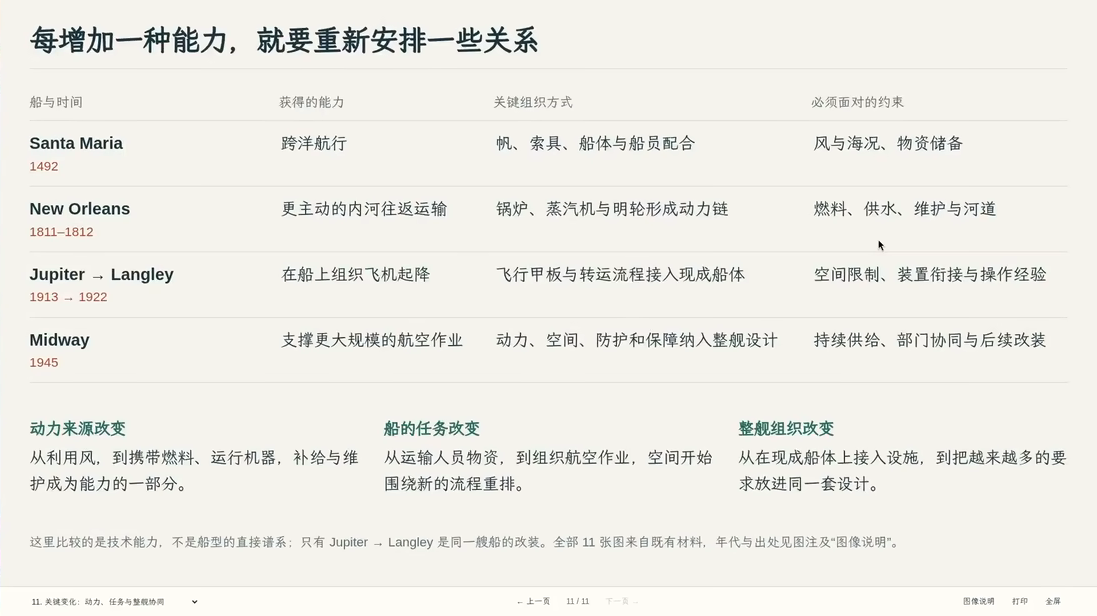
\includegraphics[width=0.92\textwidth]{figures/fig_20_ship_evolution_table.png}
\caption{四代舰船演化总结：每增加一种能力，就要重新安排动力来源、船的任务与整舰组织关系\vtag}
\end{figure}
\srcnote{00:35:30--00:35:45}

\begin{table}[H]
\centering
\small
\caption{从风帆到现代航母的四代舰船系统演化对比表}
\begin{tabular}{p{2.6cm}p{1.6cm}p{3.0cm}p{3.4cm}p{3.2cm}}
\toprule
\textbf{代表舰船} & \textbf{年代} & \textbf{获得的核心能力} & \textbf{关键内部组织方式} & \textbf{必须面对的工程约束} \\
\midrule
\textbf{Santa Maria} & 1492年 & 跨洋远航探索 & 风帆、索具、木质船体与水手人工配合 & 外部风向海况、淡水物资储备与经验 \\
\textbf{New Orleans} & 1811--1812年 & 更主动的内河逆流往返运输 & 燃料 $\to$ 锅炉 $\to$ 蒸汽机 $\to$ 船侧明轮动力链 & 燃料消耗、锅炉供水、机械维护与河道水深 \\
\textbf{USS Jupiter $\to$ Langley} & 1913--1922年 & 在船上组织固定翼飞机起降试验 & 在现成运煤船体上架起木质飞行甲板与升降转运流程 & 原有煤舱空间限制、临时滑道衔接与起降风险 \\
\textbf{USS Midway (CV-41)} & 1945年 & 高烈度海战中持续大规模航空作业 & 装甲飞行甲板、机库、多锅炉动力、损管防护整舰协同设计 & 全舰管网持续供给、多部门手册协同与喷气时代改装 \\
\bottomrule
\end{tabular}
\end{table}

在讲完航母的故事后，蒋老师展示了自己团队正在推进的“造航母”计划——构建下一代智能体操作系统（AgentOS），向全栈能力突出的同学发出招募邀请（图 21），并指出 AI 时代软件演化与传统造船的一点关键分野：
\begin{itemize}
    \item \textbf{传统物理工程}：因为钢铁与船坞试错成本极高，每次只能走极小的保守步长 $\Delta$（先造明轮船，再造运煤船，再改兰利号）。
    \item \textbf{AI 生成式软件工程}：借助推理大模型极低的原型生成成本，我们可以先让 AI \textbf{大跨步向前跳 10 步}，在几天内拼出一个类似“兰利号”的粗糙 MVP 验证未来方向是否可行；一旦探明“飞行甲板”确实是未来，再\textbf{果断回退（Revert / Reset）到干净的起点}，用建造“中途岛号”的严谨架构、模块化边界与自动化门禁一步步稳扎稳打地推进演化。
\end{itemize}

\begin{figure}[H]
\centering
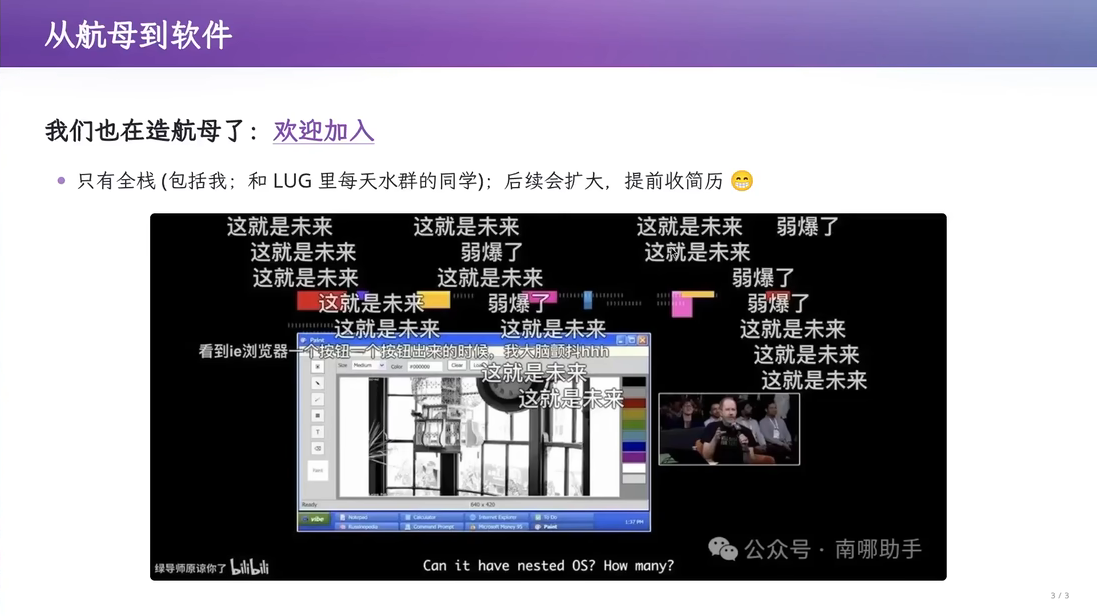
\includegraphics[width=0.92\textwidth]{figures/fig_21_building_agent_os.png}
\caption{从航母到软件：主讲团队构建下一代 AgentOS（浏览器内嵌完整桌面与智能体协同生态）的探索与招募\vtag}
\end{figure}
\srcnote{00:36:30--00:36:45}

\subsection{本章小结}

本章通过 1492年圣玛丽亚号、1811年新奥尔良号、1922年兰利号与 1945年中途岛号的四代演化史，证明了任何超级工程都是从最小可行原型（运煤船加装甲板）出发，在解决内部转运瓶颈与外部任务需求的过程中逐步重排系统关系的产物。这一历史视角为我们理解大型软件仓库的演化奠定了直观的物理图景。

% =========================================================================
% SECTION 4
% =========================================================================
\section{软件的“时间维度”：Parnas 模块化边界与 Git Rebase 学习法}

将视野从钢铁舰船拉回代码世界，软件系统同样生活在\textbf{“时间维度”}之中（图 22）。几乎所有伟大的开源软件在诞生第一天都只是一个极其精简的 Idea：Linus Torvalds 最初写 Linux 0.01 只是为了在自己的 386 机器上跑一个免费的终端仿真与类 Unix 内核；Guido van Rossum 设计 Python 最初只是为了在圣诞假期写一门比 C 语言更易读、比 Shell 脚本更结构化的胶水语言。

\begin{figure}[H]
\centering
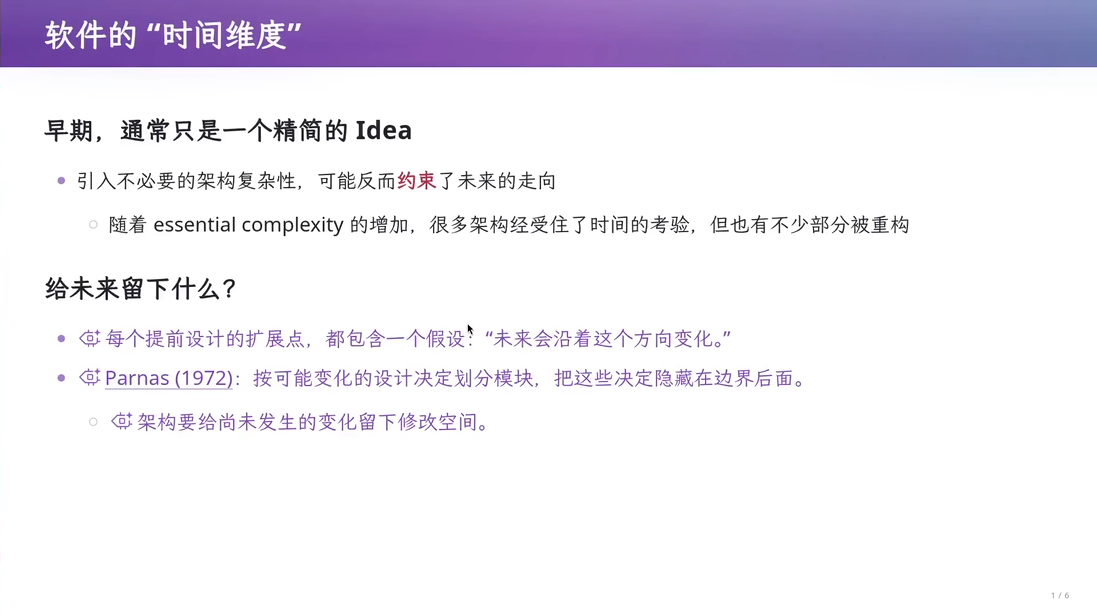
\includegraphics[width=0.92\textwidth]{figures/fig_22_software_time_dimension.png}
\caption{软件的“时间维度”：早期通常只是一个精简的 Idea；过早引入不必要的扩展点反而会约束未来走向，Parnas（1972）信息隐藏原则揭示了模块边界的本质\vtag}
\end{figure}
\srcnote{00:38:00--00:38:15}

\subsection{Parnas（1972）信息隐藏原则：为什么 Linux 换调度器易、Python 换 \texttt{print} 难？}

在软件工程教育中，初学者常被教导要“面向未来设计、预留丰富的扩展点（Extension Points）”。但蒋老师一针见血地指出：\textbf{每一个提前设计的扩展点，本质上都隐含了一个强烈的赌博假设——“未来需求一定会沿着我预留的这个方向变化”}。如果未来需求正巧沿着该方向演进，扩展点固然显得有先见之明；但只要业务方向发生正交偏转，当初精心设计的抽象层反而会变成阻碍重构的沉重枷锁。

早在 1972 年，软件工程大师大卫·帕纳斯（David L. Parnas）在经典论文《On the Criteria To Be Used in Decomposing Systems into Modules》中就给出了模块划分的黄金准则：\textbf{不要按执行流程图（Flowchart）的步骤划分模块，而应当按“未来可能发生变化的设计决定（Design Decisions Likely to Change）”划分模块，并把这些容易变化的决定严格隐藏在稳定的模块接口边界后面（Information Hiding）}。

为了验证 Parnas（1972）准则在数十年时间尺度上的威力，课堂对比了开源史上两个极其鲜明的正反案例（图 23）：

\begin{figure}[H]
\centering
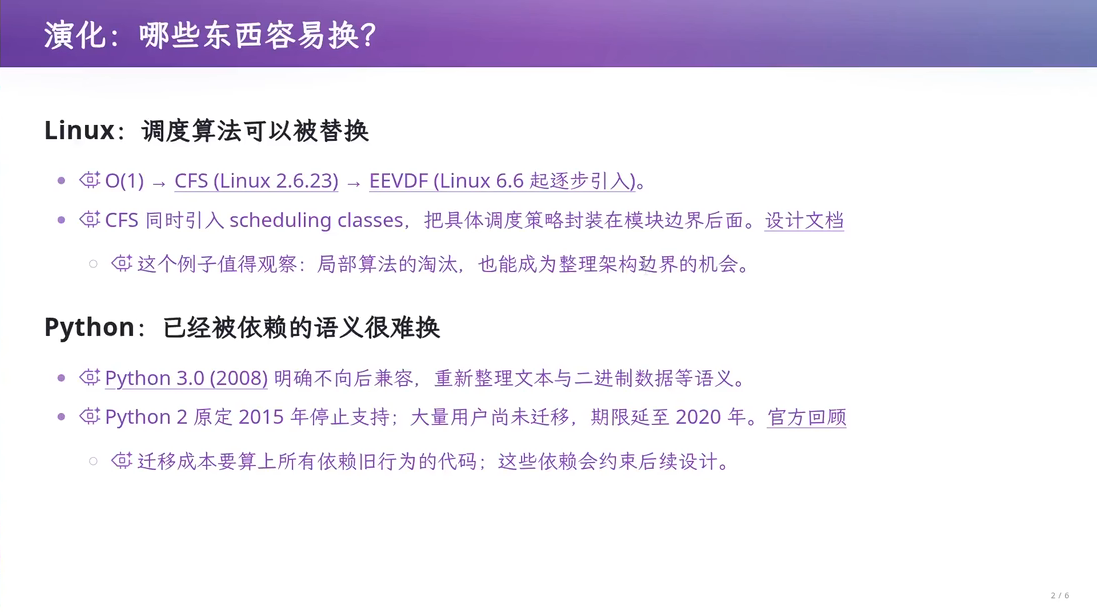
\includegraphics[width=0.92\textwidth]{figures/fig_23_easy_vs_hard_change.png}
\caption{软件演化中哪些东西容易换、哪些难换：Linux 内核调度器的三次平滑更替，对比 Python 2 到 Python 3（2008--2020）长达十二年的痛苦语义迁移\vtag}
\end{figure}
\srcnote{00:41:00--00:41:15}

\begin{enumerate}
    \item \textbf{容易替换的典范——Linux 内核进程调度器（Scheduler）}：
    在过去二十余年里，Linux 内核的主力进程调度算法经历了三次彻底的推倒重来：从 Linux 2.6 早期的 \textbf{$O(1)$ 调度器}（Ingo Moln\'{a}r 设计），到 Linux 2.6.23 引入基于红黑树虚拟运行时间的\textbf{完全公平调度器（CFS，Completely Fair Scheduler）}，再到 Linux 6.6 起逐步引入并替换 CFS 的\textbf{最早合格虚拟截止时间优先调度器（EEVDF，Earliest Eligible Virtual Deadline First）}。为什么如此核心的内核算法可以换得如此丝滑，以至于全世界数以亿计的 Linux 服务器与 Android 应用几乎完全无感？因为 CFS 在引入时顺手抽象出了清晰的 \texttt{struct sched\_class}（调度类模块边界），把具体的就绪队列数据结构与时间片算术死死关在模块内部，对上层系统调用与进程管理只暴露极简的状态钩子。
    \item \textbf{极难替换的反例——Python 2 到 Python 3 的语法与字符串语义}：
    Python 早期为了方便新手，将 \texttt{print "hello"} 设计为不带括号的语法关键字语句（Statement），并将 ASCII 字节流与文本字符串混同为 \texttt{str}。到了 2008 年，Python 3.0 痛下决心打破向后兼容，将 \texttt{print()} 统一为普通内置函数，并严格区分文本字符串（\texttt{str}）与二进制字节串（\texttt{bytes}）。这在语言设计上无疑是正确的演进，但由于 \texttt{print} 与字符串语义早已暴露在模块边界之外、渗透进全球数百万个第三方库的每一行代码中，这场迁移演变成了一场漫长的拉锯战：Python 2 原定于 2015 年停止维护（EOL），因大量工业界代码未能完成迁移而被迫延期五年，直到 2020 年才真正终结——整整耗费了十二年时间！
\end{enumerate}

\begin{warningbox}{架构反模式警示：过早抽象与错误扩展点的代价}
如果不理解业务在时间维度上的真实变化方向，而在项目第 1 天就照搬复杂的微服务拆分或十层设计模式，无异于在 1492年的木帆船上预先焊死一套错误的蒸汽管道。Parnas（1972）信息隐藏原则的精髓不在于“把所有代码都包一层接口”，而在于精准识别哪些设计决定最可能随时间改变，并用最薄的契约将其隔离。
\end{warningbox}

\subsection{软件作为状态机与“Git Rebase 冲突学习法”}

无论一个软件仓库今天膨胀到几百万行代码，从版本控制（Git）的视角来看，它依然是一个严格的\textbf{确定性状态机（State Machine）}（图 24）：每一次提交（\texttt{fix}, \texttt{feature}, \texttt{chore}, \texttt{refactor}）都是一个转移算子 $\Delta_t$，推动代码库状态从 $S_{t-1}$ 演化到 $S_t$。

\begin{figure}[H]
\centering
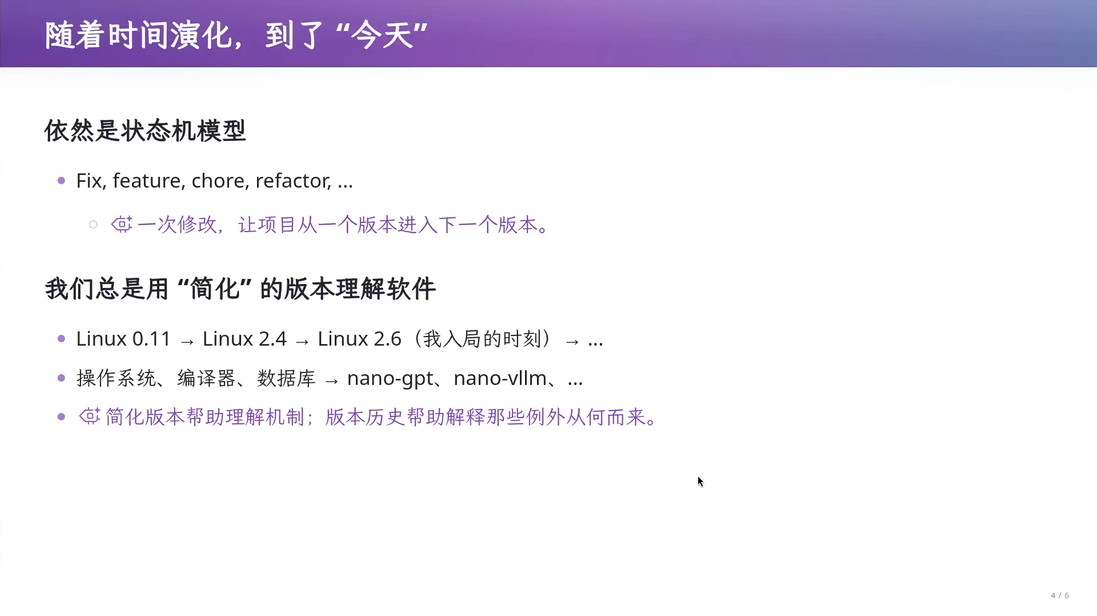
\includegraphics[width=0.92\textwidth]{figures/fig_24_state_machine_rebase.png}
\caption{随着时间演化到了“今天”：软件依然是状态机模型；用简化版本（如 Linux 0.11、\texttt{nano-gpt}、\texttt{nano-vllm}）理解核心机制，用版本历史解释例外从何而来\vtag}
\end{figure}
\srcnote{00:41:45--00:42:00}

这给我们阅读和学习超大型工业级开源项目（如现代 Linux 6.x、vLLM、Chromium）提供了一个绝妙的方法论。为什么直接去读今天的 Linux 6.x 源码会让人头晕目眩？因为今天的代码里只有 10\% 是核心机制，剩下 90\% 全是过去三十年为了兼容奇葩硬件、修复并发死锁、防御侧信道攻击而打上的历史补丁（例外处理）。

为此，蒋老师在黑板上详细推演了独创的\textbf{“Git Rebase 冲突学习法”}（图 25）：

\begin{figure}[H]
\centering
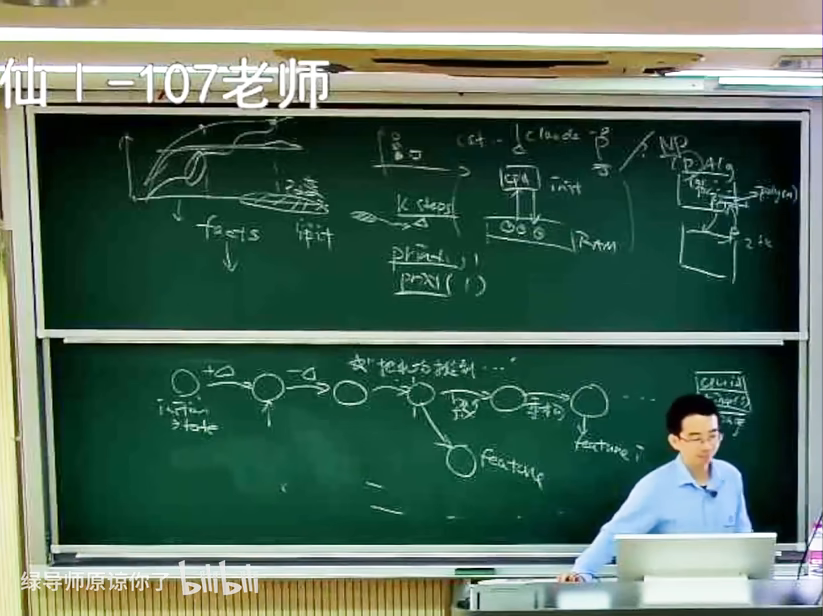
\includegraphics[width=0.88\textwidth]{figures/fig_25_board_rebase_vvar.png}
\caption{课堂板书全景：下方展示从初始状态（Initial State）沿 $+\Delta$ 演化的状态机链条，以及在早期版本实现 \texttt{cpu id / time} 共享物理页特性后向后续主干执行 \texttt{git rebase} 的冲突检测模型\vtag}
\end{figure}
\srcnote{00:48:30--00:48:45}

我们可以将这一学习法形式化为离散状态机上的交换律检验（Commutativity Check of State Transitions）：

\begin{equation}
S_t = \delta(S_{t-1}, \Delta_t), \qquad
\mathcal{C}(F, \Delta_t) = \bigl\|\delta\bigl(\delta(S_{t-1}, F), \Delta_t\bigr) - \delta\bigl(\delta(S_{t-1}, \Delta_t), F\bigr)\bigr\|
\end{equation}

其中各符号的工程含义如下：
\begin{itemize}
    \item $S_{t-1}, S_t$：代码仓库在第 $t-1$ 个版本与第 $t$ 个版本时的完整抽象语法树与文件状态；
    \item $\Delta_t$：主干演化历史上的第 $t$ 次提交补丁（Commit Diff，如一次 Bug 修复或子系统重构）；
    \item $F$：学习者在早期简化版本 $S_0$（如 Linux 0.11 或 xv6）上亲手实现的一个新特性分支（Feature Patch）；
    \item $\delta(S, \Delta)$：Git 应用补丁的状态转移函数；
    \item $\mathcal{C}(F, \Delta_t)$：将特性 $F$ 从版本 $S_{t-1}$ 变基（\texttt{git rebase}）到版本 $S_t$ 时产生的合并冲突度量（Merge Conflict）；当 $\mathcal{C}(F, \Delta_t) = 0$ 时说明历史提交 $\Delta_t$ 与特性 $F$ 正交，可自动快进略过；唯有当 $\mathcal{C}(F, \Delta_t) > 0$（发生冲突或测试破坏）时，该次提交 $\Delta_t$ 才真正触及了与特性 $F$ 耦合的架构演进点！
\end{itemize}

\begin{knowledgebox}{实战案例：在 Linux 0.11 上实现 \texttt{vvar/vDSO} 并向现代内核 Rebase}
假设你想深入理解现代操作系统中用于免系统调用（Syscall-free）高速读取系统时间（\texttt{gettimeofday}）与当前 CPU 编号的 \textbf{\texttt{vvar / vDSO} 共享内存机制}。直接看 Linux 6.x 的实现会被复杂的页表安全隔离与多架构宏搞晕。采用 \textbf{Git Rebase 学习法}只需三步：
\begin{enumerate}
    \item \textbf{回到纯真年代（$S_0$）}：检出只有一万多行代码的 Linux 0.11（或早期 Git 起点版本）。在这里实现“内核分配一页物理内存写入 \texttt{time} 与 \texttt{cpu\_id}，并以只读权限映射到所有用户进程地址空间”只需短短几十行代码（图 25 右下角板书方框）。
    \item \textbf{沿时间轴执行 \texttt{git rebase}}：将你的几十行特性补丁 $F$ 沿着 Linux 主干提交历史一步步向后 \texttt{rebase}。你会发现，主干上 99\% 的网卡驱动更新、文件系统修补都会自动无冲突滑过（$\mathcal{C} = 0$）。
    \item \textbf{在冲突处顿悟架构演化（$\mathcal{C} > 0$）}：突然在某一个历史 Commit 上，\texttt{git rebase} 停下来报错了！你打开那个 Commit 一看——原来是因为多核 SMP 架构引入了 Per-CPU 变量，或者是因为 Meltdown/Spectre 漏洞引入了内核页表隔离（KPTI），导致你原本简单的静态固定地址映射不再安全，必须做一次子系统重构。通过这寥寥几次冲突，你就把三十年操作系统演化的核心脉络彻底吃透了！
\end{enumerate}
\end{knowledgebox}

同时，蒋老师还对比了计算机专业学生的**“旧三大浪漫”**与 AI 时代的**“新三大浪漫”**：
\begin{itemize}
    \item \textbf{旧三大浪漫}：手写一个玩具操作系统内核（OS）、手写一个编译器（Compiler）、手写一个关系型数据库引擎（Database）。
    \item \textbf{AI 时代新三大浪漫}：精读并魔改极简大模型训练框架 \textbf{\texttt{nanoGPT}}、精读并魔改极简高吞吐推理引擎 \textbf{\texttt{nano-vLLM}}（理解 PagedAttention 与 Continuous Batching 的核心机制）、以及用几块廉价的国产 \textbf{RK3588 开发板拼装分布式多卡推理集群}。
\end{itemize}

\subsection{本章小结}

本章阐明了软件在时间维度上的演化规律：Parnas（1972）信息隐藏原则决定了模块替换的难易程度（Linux 调度器 vs Python 2/3 迁移）；而把软件视为离散状态机、先在极简版本（Linux 0.11、\texttt{nano-gpt}、\texttt{nano-vllm}）中把握核心机制，再通过 \texttt{git rebase} 观察历史演进中的冲突点，则是人类工程师穿透海量历史补丁、直抵本质复杂性的终极法宝。

% =========================================================================
% SECTION 5
% =========================================================================
\section{从 SWE-bench 到 Taste-bench：当“小事”被刷爆后如何度量工程品味？}

既然软件演化是由成千上万次微小的状态转移（Commits）加上关键时刻的架构重构共同构成的，那么今天的大语言模型在这条演化链条上究竟做到了哪一步？

\subsection{精读 ICLR 2024 经典论文：SWE-bench 的诞生与早期惨淡表现}

为了回答这一问题，蒋老师带大家回顾了普林斯顿大学 Carlos E. Jimenez、John Yang、Shunyu Yao 等人于 2023年 10 月发布、并于 ICLR 2024 正式发表的里程碑论文——\textbf{《SWE-bench: Can Language Models Resolve Real-World GitHub Issues?》}（图 26）。

\begin{figure}[H]
\centering
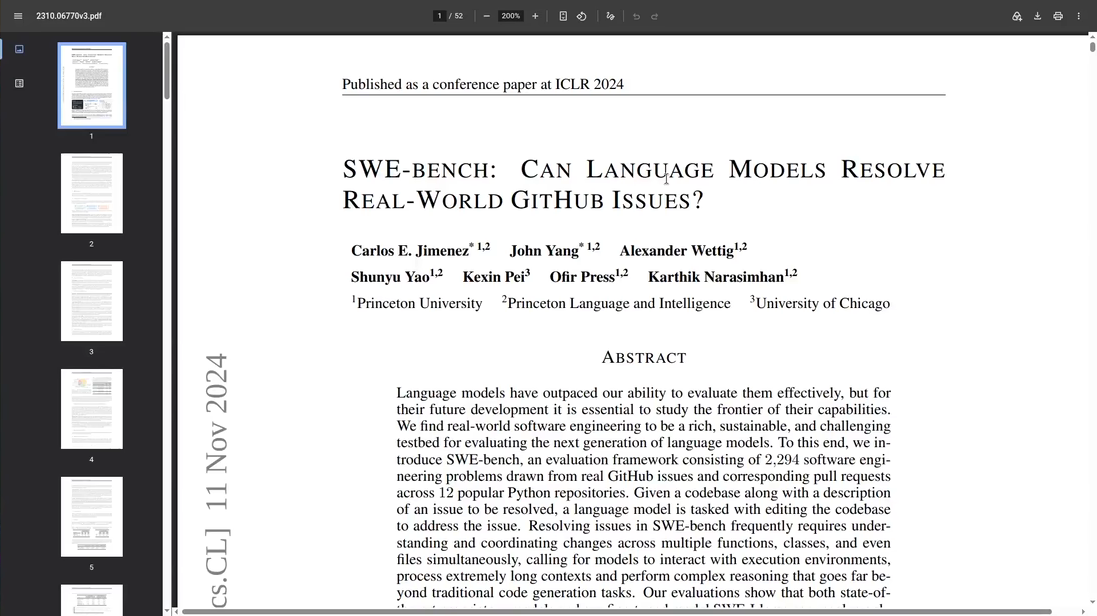
\includegraphics[width=0.92\textwidth]{figures/fig_26_swebench_paper.png}
\caption{ICLR 2024 论文《SWE-bench: Can Language Models Resolve Real-World GitHub Issues?》首页：从 12 个流行 Python 开源仓库采集 2,294 个真实工程问题\vtag}
\end{figure}
\srcnote{00:52:00--00:52:15}

在 SWE-bench 出现之前，大模型代码评测主要停留在 HumanEval 或 MBPP 这类“给定函数签名写几十行独立算法题”的玩具基准上。SWE-bench 第一次把评测场景拉到了真实的工业级软件演化历史中（图 27）：

\begin{figure}[H]
\centering
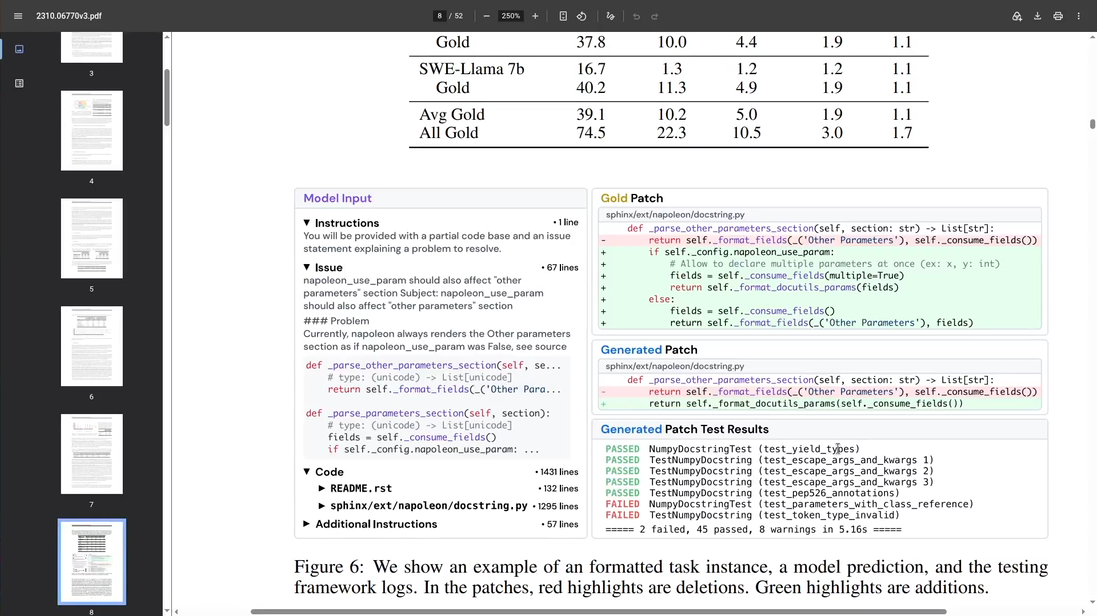
\includegraphics[width=0.92\textwidth]{figures/fig_27_swebench_workflow.png}
\caption{SWE-bench 评测实例拆解（论文 Figure 6）：给定仓库历史快照与 GitHub Issue 描述（左），对比人类开发者的 Gold Patch（右上）与模型生成的 Generated Patch 及其测试集通过结果（右下）\vtag}
\end{figure}
\srcnote{00:53:00--00:53:15}

\begin{enumerate}
    \item \textbf{数据构建方式}：从 \texttt{django}、\texttt{scikit-learn}、\texttt{matplotlib}、\texttt{sphinx}、\texttt{sympy}、\texttt{pytest}、\texttt{flask}、\texttt{requests} 等 12 个知名 Python 开源仓库中，筛选出 2,294 个真实的“GitHub Issue + 对应修复 Pull Request（PR）”配对实例。
    \item \textbf{评测闭环}：给模型提供该 PR 合并前的完整代码库快照（Codebase）以及自然语言 Issue 问题描述（如 \texttt{sphinx} 中 \texttt{napoleon\_use\_param} 配置项未对 \texttt{Other Parameters} 段落生效的 Bug）。模型必须自己跨文件检索定位代码、输出一个补丁（Generated Patch）；随后评测框架将真实 PR 中新增的单元测试（Fail-to-Pass Tests）打入容器运行——只有当原本失败的测试全部变为 \texttt{PASSED} 且不破坏原有回归测试时，才算成功解决（Resolved）。
\end{enumerate}

令人印象深刻的是，在 2023年底至 2024 年初论文发表时，当时最顶尖的大模型在 SWE-bench 面前几乎全军覆没！图 28 展示了原论文 Table 5 与 Figure 4 的真实统计数据：

\begin{figure}[H]
\centering
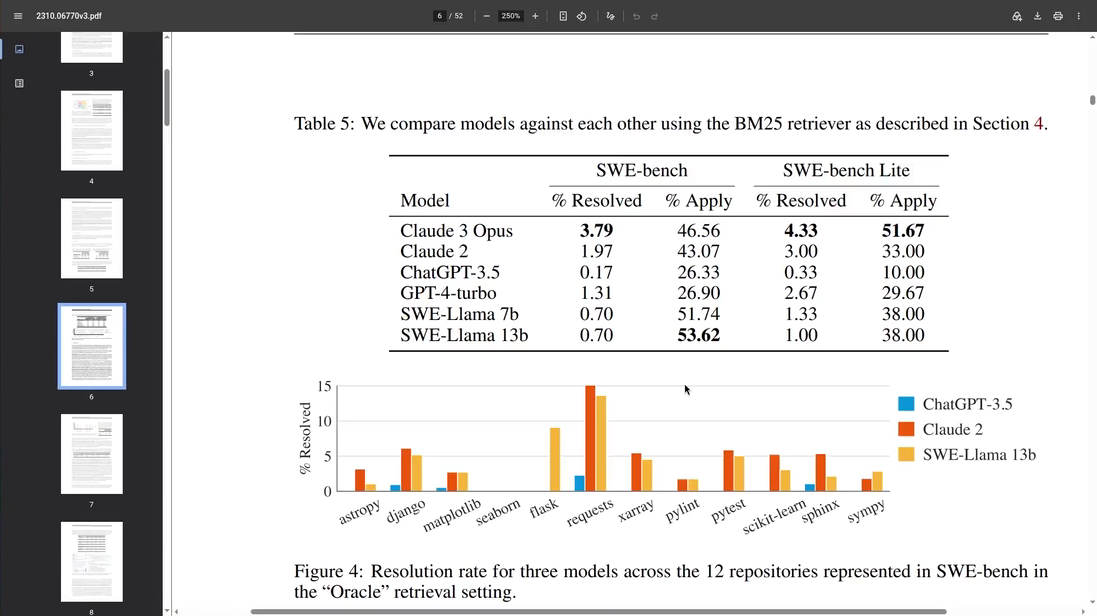
\includegraphics[width=0.92\textwidth]{figures/fig_28_swebench_table5.png}
\caption{SWE-bench 论文 Table 5 与仓库分布图（Figure 4）：在 BM25 检索设置下，Claude 3 Opus 在完整集上仅解决 3.79（Lite 4.33），GPT-4-turbo 仅解决 1.31（Lite 2.67）\vtag}
\end{figure}
\srcnote{00:53:45--00:54:00}

我们把图 28 中的核心实验结果整理为表 2，可以清晰看到当年模型哪怕生成了能打上补丁的 diff（\texttt{\% Apply} 约 26\%--53\%），真正能通过测试集的比率也微乎其微：

\begin{table}[H]
\centering
\small
\caption{SWE-bench 原始论文（Table 5，BM25 检索器设置）各模型早期解决率对比}
\begin{tabular}{p{3.2cm}p{2.3cm}p{2.6cm}p{2.3cm}p{2.6cm}}
\toprule
\textbf{评测模型} & \textbf{Full 解决率} & \textbf{Full 可应用率} & \textbf{Lite 解决率} & \textbf{Lite 可应用率} \\
\midrule
\textbf{Claude 3 Opus} & \textbf{3.79} & 46.56 & \textbf{4.33} & \textbf{51.67} \\
\textbf{Claude 2} & 1.97 & 43.07 & 3.00 & 33.00 \\
\textbf{GPT-4-turbo} & 1.31 & 26.90 & 2.67 & 29.67 \\
\textbf{SWE-Llama 13b} & 0.70 & \textbf{53.62} & 1.00 & 38.00 \\
\textbf{SWE-Llama 7b} & 0.70 & 51.74 & 1.33 & 38.00 \\
\textbf{ChatGPT-3.5} & 0.17 & 26.33 & 0.33 & 10.00 \\
\bottomrule
\end{tabular}
\end{table}

\begin{knowledgebox}{评测基准演化规律：为什么带二值验证器的任务必然被 RL 刷爆？}
只要一个软件工程任务具备确定性的自动判题器（Verifier，如单元测试通过与否），且基础模型在该任务上的零样本采样存在非零成功概率（哪怕只有 1\%--3\%），大规模强化学习（如 GRPO 与拒绝采样微调）就能通过海量并发采样将高奖励轨迹蒸馏进权重。因此，单点 Bug 修复注定从“前沿研究问题”退化为“算力工程问题”。
\end{knowledgebox}

\subsection{从 3.79 到突破 65\%：为什么我们需要基于 Thurstone（1927）的 \texttt{Taste-bench}？}

短短一年半之后，剧情发生了翻天覆地的逆转（图 29）：到了 2025年 7 月，仅用百余行代码编写的极简智能体框架 \texttt{mini-SWE-agent} 配合新一代推理基座模型，在人工清洗后的 \textbf{SWE-bench Verified} 权威子集上就已经达到了 \textbf{65\%} 以上的解决率，而到了 2026年更是逼近饱和！

\begin{figure}[H]
\centering
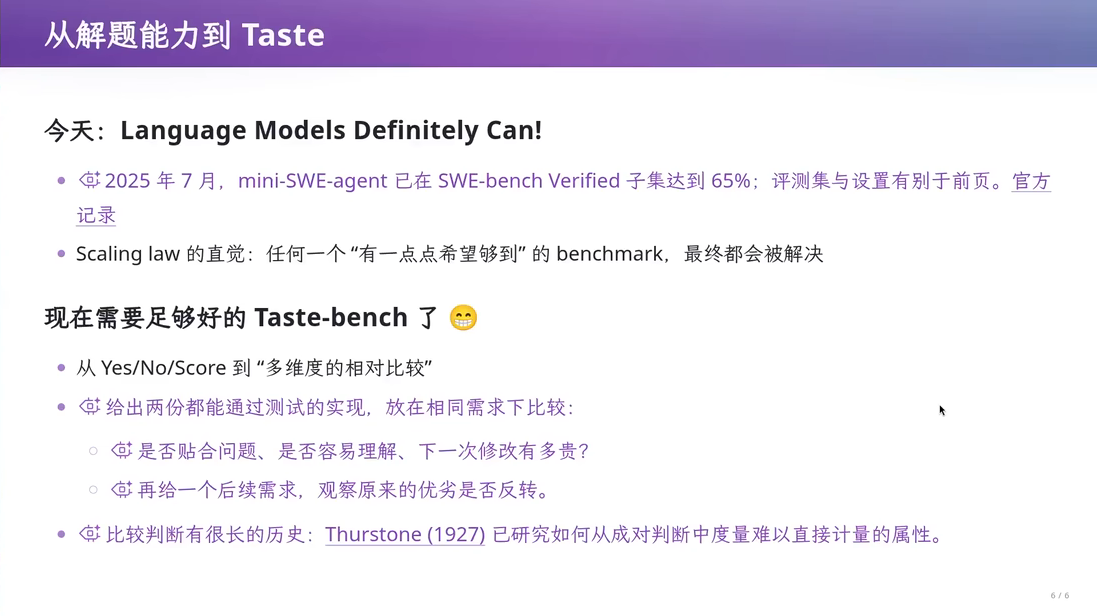
\includegraphics[width=0.92\textwidth]{figures/fig_29_from_solve_to_taste.png}
\caption{从解题能力到 Taste：2025年 7 月 \texttt{mini-SWE-agent} 在 SWE-bench Verified 子集达到 65\%；当具备二值验证信号的“小事”被攻克后，亟需引入 Thurstone（1927）成对比较判断法构建 \texttt{Taste-bench}\vtag}
\end{figure}
\srcnote{00:56:30--00:56:45}

为什么当年看似高不可攀的 SWE-bench 会被攻克得如此迅速？蒋老师总结了一条深刻的\textbf{Scaling Law 与强化学习（RLVR）直觉}：
\begin{quote}
\textbf{任何一个“有一点点希望够得着（初始非零解率 > 1\%）”且拥有确定性二值验证信号（Yes/No 测试集通过与否）的 Benchmark，最终都必然会被大规模强化学习采样彻底刷爆。}
\end{quote}

但是，SWE-bench 被刷爆是否意味着“软件工程已经被 AI 彻底解决了”？绝非如此！因为 SWE-bench 里采集的 2,294 个 Issue，本质上全都是软件演化状态机里的\textbf{“局部小事（Local Minor Steps）”}——即在现有架构框架内修一个边界条件 Bug、加一个局部配置项分支。而在真实的航母建造与大型软件演化史中，决定项目生死的恰恰是 SWE-bench 完全没有覆盖的\textbf{三件“大事”}：
\begin{enumerate}
    \item \textbf{第零步创世设计（\texttt{Initial Commit}）}：在第一行代码写下之前，如何确定微内核边界、插件通信原语与目录划分？
    \item \textbf{何时停止打补丁、果断发起子系统级重构（Refactoring Threshold）}：就像兰利号（USS Langley）的临时滑道已经无法支撑更重的舰载机时，什么时候应该停止在运煤船上敲敲打打，转而像 Linux 3.4/4.0 重写 USB 子系统、或者像 \texttt{Bun} 团队近期将核心部分从 Zig 迁移到 Rust 那样，做一次伤筋动骨的架构跃迁？
    \item \textbf{两份同样通过 100\% 测试的代码，哪一份更有“品味（Taste）”？}
\end{enumerate}

为了度量难以用单一单元测试给出 \texttt{PASS/FAIL} 的工程品味，蒋老师呼吁学术界与工业界共同构建下一代基准——\textbf{\texttt{Taste-bench}}（图 29 下半部分）：
\begin{itemize}
    \item \textbf{双实现同台竞技}：给定同一个需求，让两个模型（或两个架构方案）各自生成一份\textbf{都能 100\% 通过当前功能测试}的代码实现 $A$ 与 $B$。
    \item \textbf{引入时间维度的后续需求反转检验}：不仅静态比较 $A$ 和 $B$“是否贴合问题本质、是否容易被人类理解、修改代价有多高”，更关键的是\textbf{紧接着注入第 $t+1$ 步的真实演化需求 $\Delta_{t+1}$}，观察在实现后续需求时，$A$ 与 $B$ 的修改行数、模块侵入度以及优劣评价是否发生戏剧性反转！
    \item \textbf{Thurstone（1927）比较判断定律（Law of Comparative Judgment）}：心理物理学先驱路易斯·瑟斯顿（Louis Leon Thurstone）早在 1927 年就证明，对于“审美、品味、字迹优美度”这类难以直接用标尺给出绝对分数的属性，只要收集大量受试者在成对比较（Pairwise Comparison）中的胜负概率，就能通过统计模型反推出潜在的连续质量标度：
\end{itemize}

\begin{equation}
P(A \succ B \mid d) = \Phi\!\left(\frac{\mu_{A,d} - \mu_{B,d}}{\sqrt{\sigma_{A,d}^2 + \sigma_{B,d}^2}}\right), \qquad
\mathbf{T}(A) = \bigl(\mu_{A,1}, \mu_{A,2}, \dots, \mu_{A,D}\bigr)^{\top}
\end{equation}

其中各符号的含义如下：
\begin{itemize}
    \item $P(A \succ B \mid d)$：在给定的第 $d$ 个工程质量维度（如可读性、状态内聚性、对未来需求 $\Delta_{t+1}$ 的扩展弹性）上，代码实现 $A$ 被评审者（或演化压力测试）判定优于实现 $B$ 的概率；
    \item $\mu_{A,d}, \mu_{B,d}$：代码实现 $A$ 与 $B$ 在第 $d$ 个品味维度上的潜在真实质量均值（Latent Taste Score）；
    \item $\sigma_{A,d}^2, \sigma_{B,d}^2$：两种实现在单次采样或特定任务上下文下的表现方差（表征发挥稳定性）；
    \item $\Phi(\cdot)$：标准正态分布的累积分布函数（或简化为 Bradley-Terry / Elo 模型中的 Sigmoid 函数 $\sigma(z) = (1 + e^{-z})^{-1}$）；
    \item $\mathbf{T}(A) \in \mathbb{R}^D$：不同于传统排行榜压缩成单一标量总分，\texttt{Taste-bench} 应当输出一个保留帕累托权衡特征的\textbf{多维品味向量（Multi-dimensional Taste Vector）}。
\end{itemize}

\subsection{本章小结}

本章通过精读 ICLR 2024 的 SWE-bench 论文，对比了从早期 Claude 3 Opus（3.79）与 GPT-4-turbo（1.31）到 2025年 7 月 \texttt{mini-SWE-agent} 突破 65\% 的技术跃迁，指出具备二值验证信号的局部编码任务已被强化学习攻克。未来的核心战场在于构建基于 Thurstone（1927）成对比较判断法与后续需求演化压力测试的 \textbf{\texttt{Taste-bench}}，将评测重心从“能不能跑通测试”升级为“能不能经受住时间维度的演化考验”。

% =========================================================================
% SECTION 6
% =========================================================================
\section{DeepSeek Harness 真实演化史：前 1,000 个提交与四大工程宝藏}

理论剖析之后，本讲进入了最受期待的实战考古环节：既然上一讲我们静态拆解了 \texttt{DeepSeek Harness (dsh)} 的微内核架构，那么\textbf{这艘智能体时代的“中途岛号航母”，究竟是如何在短短几个月内从第 1 次 Git 提交一步步长成今天这副模样的？}

蒋老师盛赞了 DeepSeek 团队的开源诚意（图 30）：不同于许多大厂开源项目在发布前把内部研发历史全部压扁（Squash）成一个冷冰冰的 \texttt{Initial public release} 提交，\texttt{dsh} 仓库\textbf{原汁原味地保留了从项目诞生第一天（2026年 6 月 10 日）起的全部两万两千多个 Git Commits}！这为我们提供了一座研究生成式软件工程演化的无价富矿。

\begin{figure}[H]
\centering
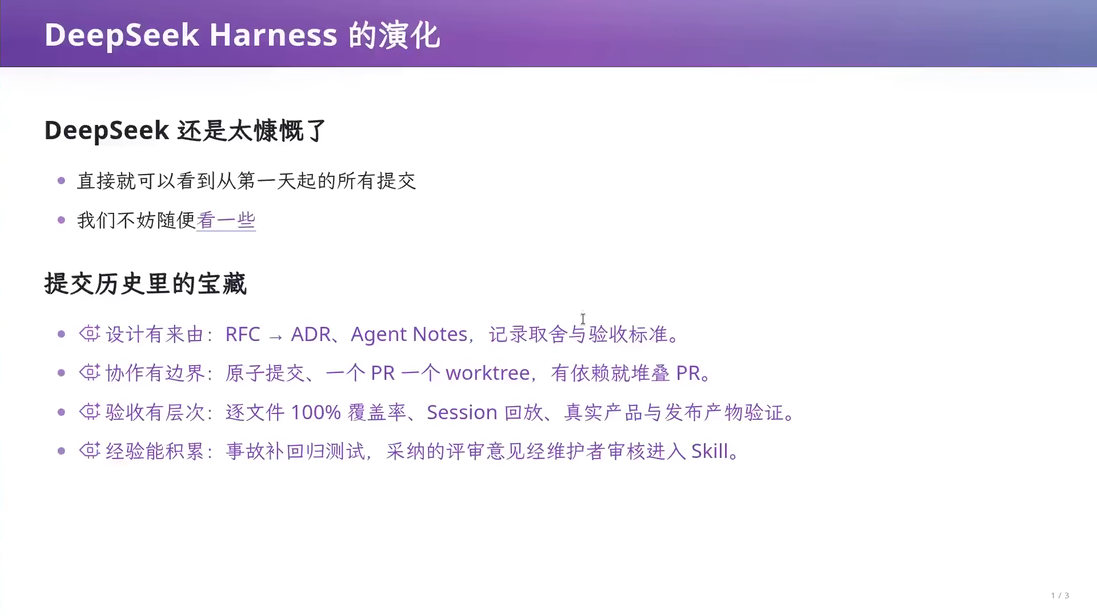
\includegraphics[width=0.92\textwidth]{figures/fig_30_dsh_evolution_gems.png}
\caption{DeepSeek Harness 的演化：完整保留从第一天起的全部提交历史，蕴含设计有来由、协作有边界、验收有层次、经验能积累四大工程宝藏\vtag}
\end{figure}
\srcnote{01:04:45--01:05:00}

\subsection{前 1,000 个提交考古：从 Cordis 汇入、10天地基到 Web 浏览器甲板跃迁}

通过课堂现场的雙栏终端与网页讲义（图 31、图 32），蒋老师带大家逐一检视了 \texttt{dsh} 仓库最早的提交记录（从第 1 个提交 \texttt{b67e81ac97} 到第 1000 个提交 \texttt{a7b569850b}，按每 25 个提交一组划分为 40 组）：

\begin{figure}[H]
\centering
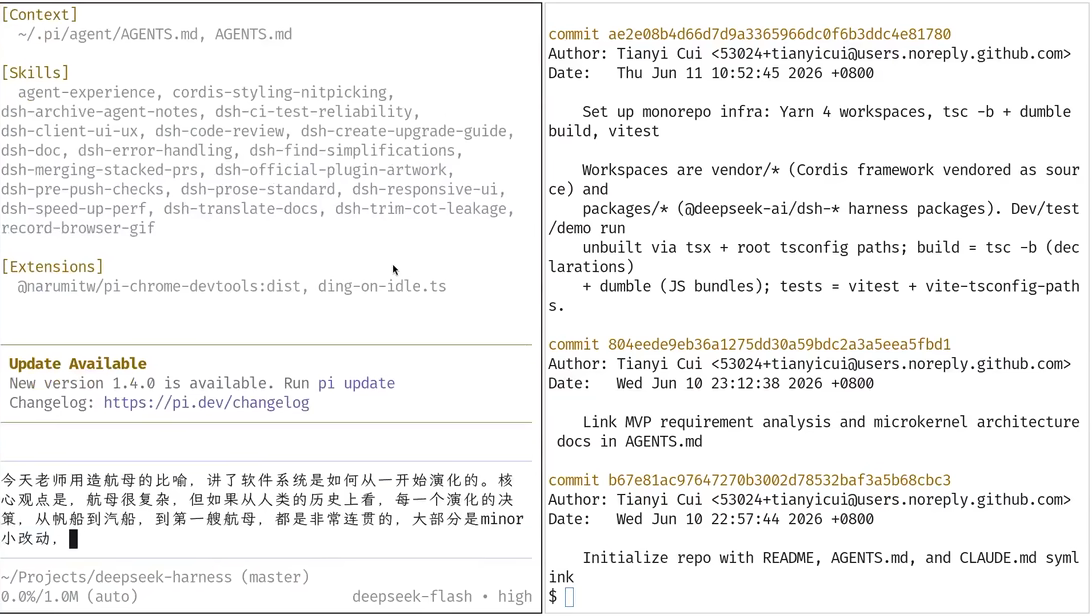
\includegraphics[width=0.92\textwidth]{figures/fig_31_dsh_first_1000_part1.png}
\caption{DeepSeek Harness 最早提交终端实录：左栏展示加载的 15 个核心工程 Skills（含 \texttt{dsh-prose-standard}、\texttt{dsh-pre-push-checks} 等），右栏展示 2026年 6 月 10 日至 11 日的前三次创世提交\vtag}
\end{figure}
\srcnote{01:06:00--01:06:15}

\begin{figure}[H]
\centering
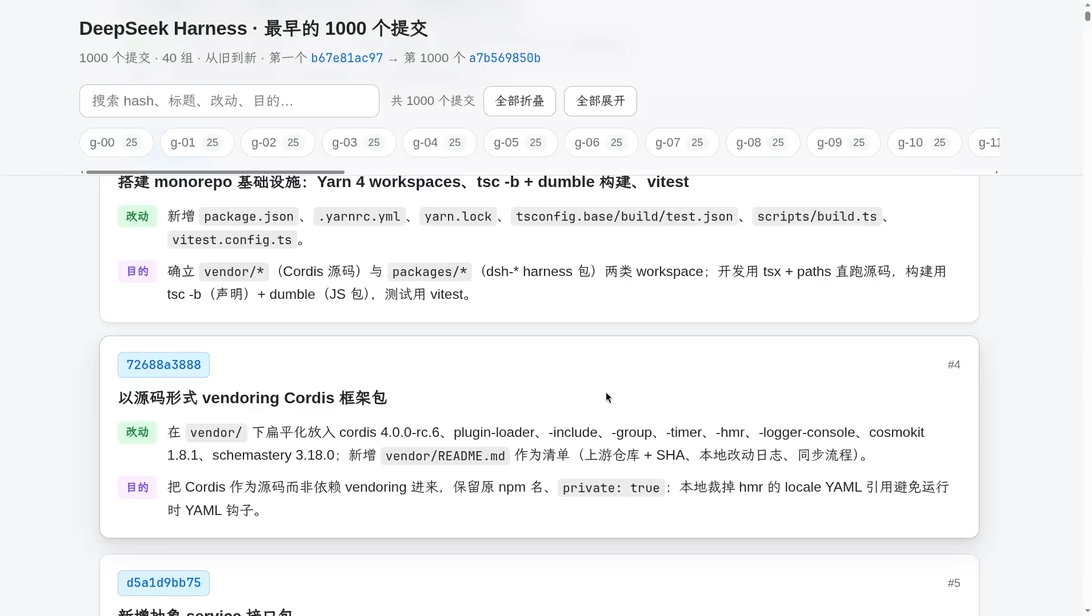
\includegraphics[width=0.92\textwidth]{figures/fig_32_dsh_first_1000_part2.png}
\caption{DeepSeek Harness 最早的 1,000 个提交考古（\texttt{b67e81ac97} $\to$ \texttt{a7b569850b}）：第 3 个提交搭建 Yarn 4 Monorepo 基础设施，第 4 个提交（\texttt{72688a3888}）以源码形式 vendoring 汇入 Cordis 框架包\vtag}
\end{figure}
\srcnote{01:07:30--01:07:45}

观察前 1,000 个提交的演进脉络，可以清晰地看到一艘“软件航母”建造的四个关键阶段：

\begin{enumerate}
    \item \textbf{创世前 4 步（2026年 6 月 10 日--11 日）——先立规矩与微内核底座，再写业务代码}：
    \begin{itemize}
        \item \textbf{Commit \#1（\texttt{b67e81ac97}，6 月 10 日 22:57）}：\texttt{Initialize repo with README, AGENTS.md, and CLAUDE.md symlink}。注意！项目第一行代码还没写，第一件事是初始化指导智能体协作的 \texttt{AGENTS.md} 宪章！
        \item \textbf{Commit \#2（\texttt{804eede9eb}，6 月 10 日 23:12）}：\texttt{Link MVP requirement analysis and microkernel architecture docs in AGENTS.md}。仅隔 15 分钟，立刻将 MVP 需求分析与微内核架构设计文档挂载进 \texttt{AGENTS.md}，确保后续每一个被唤醒的 AI Agent 都共享同一套架构蓝图。
        \item \textbf{Commit \#3（\texttt{ae2e08b4d6}，6 月 11 日 10:52）}：搭建 Monorepo 基础设施（Yarn 4 workspaces、\texttt{tsc -b} 类型声明构建、\texttt{dumble} JS 打包与 \texttt{vitest} 测试框架），严格确立 \texttt{vendor/*} 与 \texttt{packages/*} 两类工作区。
        \item \textbf{Commit \#4（\texttt{72688a3888}）}：\textbf{以源码形式 vendoring 汇入 Cordis 框架包}（在 \texttt{vendor/} 下扁平化放入 \texttt{cordis 4.0.0-rc.6}、\texttt{plugin-loader}、\texttt{hmr}、\texttt{schemastery 3.18.0} 等，并裁掉冗余的 YAML 钩子）。蒋老师特别感慨：Cordis 原本是开源社区个人开发者（Shigma）为了管理聊天机器人（Koishi）插件生命周期而打磨多年的依赖注入与控制反转框架；DeepSeek 架构师凭借深厚的技术视野将其识别出来，通过源码 vendoring 改造成智能体操作系统的微内核总线——这正是“把成熟的蒸汽机装进新船体”的绝佳写照！
    \end{itemize}
    \item \textbf{第一阶段（前 10天，6 月 10 日--6 月 20 日）——筑牢可回放会话与 Agent Loop 地基}：
    在项目启动的最初 10天里，团队没有急着堆砌花哨的界面，而是集中火力攻克了 \textbf{Event Sourcing（事件溯源）会话模型（Session）}与核心 \textbf{Agent Loop}：让智能体的每一次思考、每一次工具调用、每一次状态变更都作为不可变事件（Immutable Event）持久化记录下来，天然支持任意时间点的确定性回放（Replay）与分支分叉（Fork）。
    \item \textbf{第二阶段（6 月下旬--7 月中旬）——把外部世界关进可控的插件笼子}：
    紧接着，团队将文件系统读写、子进程生成、伪终端（PTY）、语言服务器协议（LSP）等高危外部能力逐一封装为标准化的 Cordis Service 插件，并在插件边界上加装严格的权限护栏（Guardrails）与超时熔断机制。
    \item \textbf{第三阶段（7 月 19 日--8 月 6 日）——从终端 TUI 到 Web 浏览器甲板的战略跃迁}：
    这是整个 \texttt{dsh} 演化史上最像“运煤船加装飞行甲板（Jupiter $\to$ Langley）”的决定性时刻！最初的 \texttt{dsh} 与 Claude Code 类似，运行在字符终端（Terminal UI）里；但到了 7 月中旬，团队敏锐意识到终端字符网格极大限制了智能体与人类的富媒体交互带宽。于是从 7 月 19 日到 8 月 6 日，团队果断发起架构跃迁，将主交互面迁移到\textbf{Web 浏览器（DOM 树 + 命名插槽 Slots）}之上，让每一个插件不仅能注册后端工具，还能向浏览器前端动态注入响应式 UI 组件。这一跃迁直接催生了后来惊艳全场的 \textbf{\texttt{Creator Mode}（智能体实时修改并热重载宿主界面本身）}！
\end{enumerate}

\begin{importantbox}{从 TUI 到 Web 浏览器甲板：把握架构演化的“兰利号时刻”}
DeepSeek Harness 在前 10天筑牢 Event Sourcing 会话地基后，于 7 月 19 日至 8 月 6 日果断将交互甲板从字符终端（TUI）迁移至 Web 浏览器（DOM + Slots）。这次战略跃迁如同把运煤船改装为兰利号航母：由于底层 Cordis 微内核与会话状态机封装良好，上层交互界面的彻底重构非但没有伤及筋骨，反而解锁了智能体自修改宿主界面的 \texttt{Creator Mode}。
\end{importantbox}

\subsection{提交历史里的四大工程宝藏与仓库规模实测}

除了宏观路线图，蒋老师还深入挖掘了 \texttt{dsh} 提交历史中支撑“人机混合军团”高速运转而不崩盘的\textbf{四大工程宝藏}（图 30、图 33、图 34）：

\begin{figure}[H]
\centering
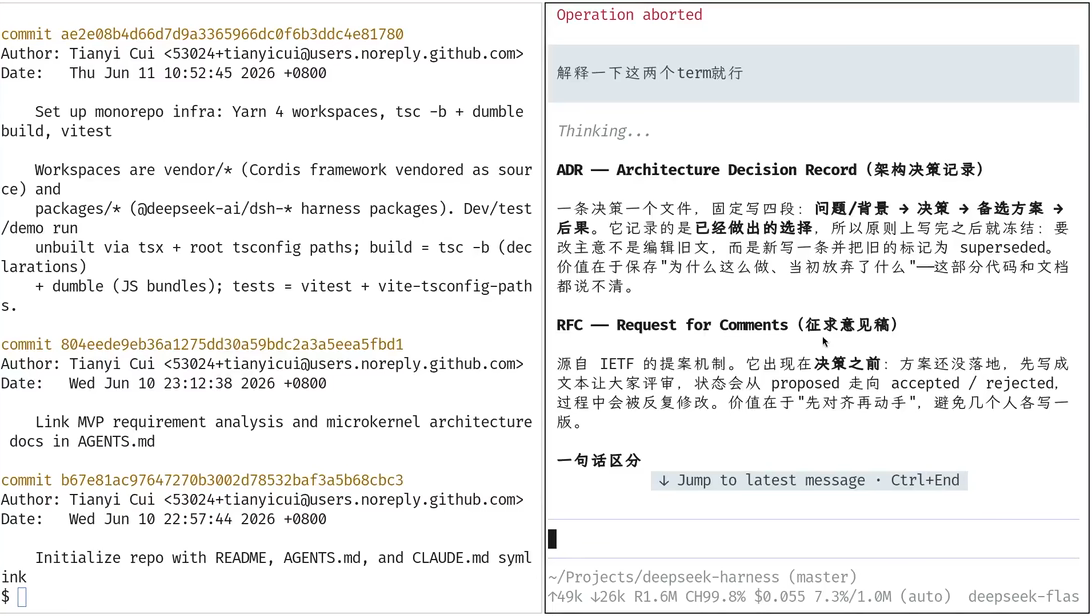
\includegraphics[width=0.92\textwidth]{figures/fig_33_rfc_to_adr_example.png}
\caption{源码仓库考古双栏对照：左栏为仓库早期提交日志，右栏剖析 \texttt{RFC}（征求意见稿，决策前反复修改对齐）与 \texttt{ADR}（架构决策记录，决策后四段式冻结归档）的职责分工\vtag}
\end{figure}
\srcnote{01:13:15--01:13:30}

\begin{enumerate}
    \item \textbf{宝藏一：设计有来由（\texttt{RFC $\to$ ADR $\to$ Agent Notes} 完整证据链）}：
    为什么我们平时读别人的代码总是搞不懂“他当年为什么要这么写，而不是用更简单的方案 B”？因为代码本身只保留了最终结果，丢掉了被否决的备选方案。在 \texttt{dsh} 仓库中（图 33 右栏）：
    \begin{itemize}
        \item \textbf{\texttt{RFC}（Request for Comments，征求意见稿）}：源自互联网工程任务组（IETF）的提案机制，出现在\textbf{重大决策落地之前}。当需要重构某个跨包机制（例如课堂展示的 9 月 5 日提案：原本 \texttt{System Prompt} 被放在每次请求的临时 Header/参数里传递，导致回放 Session 时丢失系统提示词上下文；提案将其统一迁入 \texttt{Session} 事件流持久化）时，先写成 RFC 文本评审，状态从 \texttt{proposed} 走向 \texttt{accepted / rejected}，实现“先对齐再动手”。
        \item \textbf{\texttt{ADR}（Architecture Decision Record，架构决策记录）}：出现在\textbf{决策拍板之后}。一条决策对应一个独立编号文件，固定采用四段式结构：\textbf{问题/背景 $\to$ 决策 $\to$ 备选方案（Alternatives Considered） $\to$ 后果（Consequences）}。ADR 原则上写完即\textbf{冻结（Immutable）}：未来如果改主意，绝不回滚编辑旧文，而是新写一条 ADR 并将旧文档标记为 \texttt{superseded}。这让任何人类或 AI Agent 在半年后接手代码时，都能瞬间查清历史取舍的全部因果。
    \end{itemize}
    \item \textbf{宝藏二：协作有边界（原子提交、单 PR 单 Worktree、堆叠 PR）}：
    在 AI 智能体并发编程时，最怕多个任务在同一个工作目录里互相污染未提交的文件。因此 \texttt{dsh} 严格执行**“一个任务 = 一个独立 Git Worktree = 一个原子 PR”**；若任务 B 依赖尚未合并的任务 A，则采用\textbf{堆叠 PR（Stacked PRs，配有专门的 \texttt{dsh-merging-stacked-prs} 技能）}保持主干分支极度清晰。
    \item \textbf{宝藏三：验收有层次（逐文件 100\% 覆盖率 + Session 回放 + 产物核验）}：
    不仅要求单元测试通过，而且在关键核心包上强制要求\textbf{逐文件 100\% 测试覆盖率}，配合真实 Session 录制回放与构建产物（Bundle）完整性校验。
    \item \textbf{宝藏四：经验能积累（事故补回归测试，评审意见升格进 Skill）}：
    每当线上或开发过程中发生一次 Bug 事故，不仅要补上回归测试，而且在 Code Review 中被采纳的高价值架构评审意见，会经过核心维护者（Maintainer）审核后\textbf{正式写入项目的工程 Skill 或静态检查脚本}，确保全团队的所有 AI 智能体永远不再犯同类错误。
\end{enumerate}

图 34 与表 3 展示了课堂现场使用 \texttt{git rev-list --count HEAD} 对 \texttt{dsh} 仓库（截至 \texttt{HEAD = 687f282e86}）进行的精确规模测算（注：课堂口述时曾近似提及约 22,000 或 22,580 次提交、2,340 个代码文件与 3,540 个测试文件，终端实测精确提交总数为 \textbf{22,395} 次）：

\begin{figure}[H]
\centering
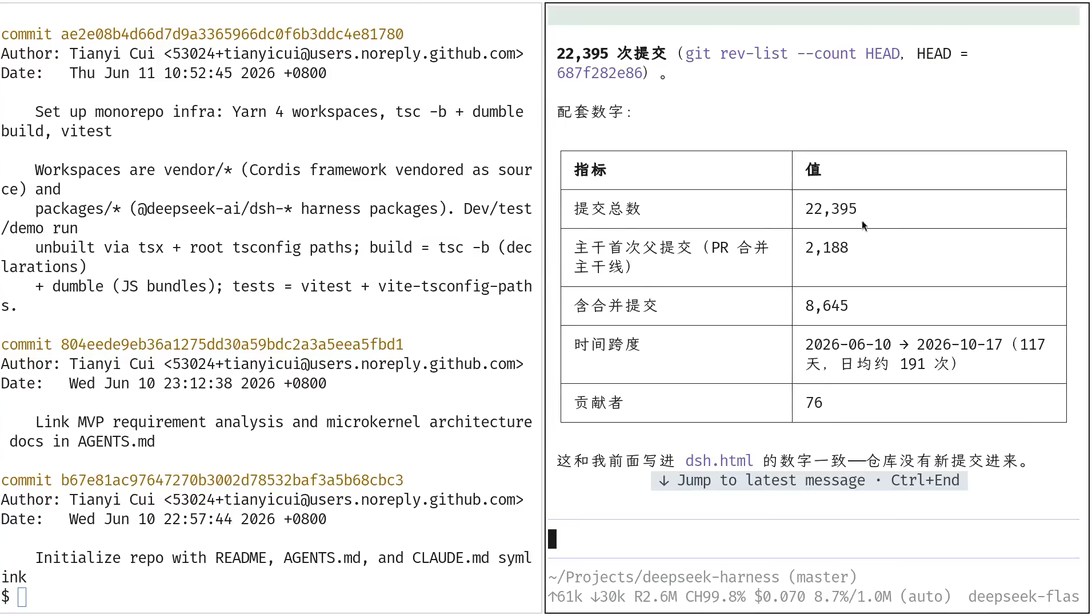
\includegraphics[width=0.92\textwidth]{figures/fig_34_dsh_repo_stats.png}
\caption{DeepSeek Harness 仓库规模实测数据（\texttt{HEAD = 687f282e86}）：117 天内累计 22,395 次 Git 提交、2,188 次主干 PR 合并、8,645 次含合并提交与 76 位贡献者\vtag}
\end{figure}
\srcnote{01:16:45--01:17:00}

\begin{table}[H]
\centering
\small
\caption{DeepSeek Harness（\texttt{dsh}）代码仓库演化规模实测统计表}
\begin{tabular}{p{3.8cm}p{3.5cm}p{5.8cm}}
\toprule
\textbf{统计维度 / 指标名称} & \textbf{实测数值} & \textbf{生成式软件工程意义解读} \\
\midrule
\textbf{Git 提交总数（Total Commits）} & 22,395 次（口述约 22,580） & 高频原子化微步提交，完整记录人机协同演化轨迹 \\
\textbf{主干首次父提交（PR 合并主干线）} & 2,188 次 & 平均每个合并到主干的 PR 包含约 10.2 个细粒度提交 \\
\textbf{含合并提交（Merge Commits）} & 8,645 次 & 支撑多分支/多 Worktree 堆叠开发与同步合流 \\
\textbf{演化时间跨度（Time Span）} & 117 天（2026-06-10 $\to$ 10-17） & 从零起步不到四个月即完成微内核与 Web 甲板迭代 \\
\textbf{日均提交频率（Daily Velocity）} & 约 191 次 / 天 & 76 位贡献者借力 Coding Agents 实现工业级高吞吐 \\
\textbf{代码与测试文件规模（课堂统计）} & 约 2,340 代码 / 3,540 测试文件 & 测试文件数显著多于业务源码文件数，构筑严密护栏 \\
\bottomrule
\end{tabular}
\end{table}

\subsection{为什么 AI 在大空间采样中仍然容易迷失方向？}

面对如此惊人的日均 191 次提交，是不是只要把需求丢给 AI 就能自动长出好系统？蒋老师立刻泼了一盆清醒的冷水：\textbf{“AI 在大空间中采样仍然非常容易迷失方向，项目总体仍然是由真人架构师牢牢掌舵的！”}（图 35）

\begin{figure}[H]
\centering
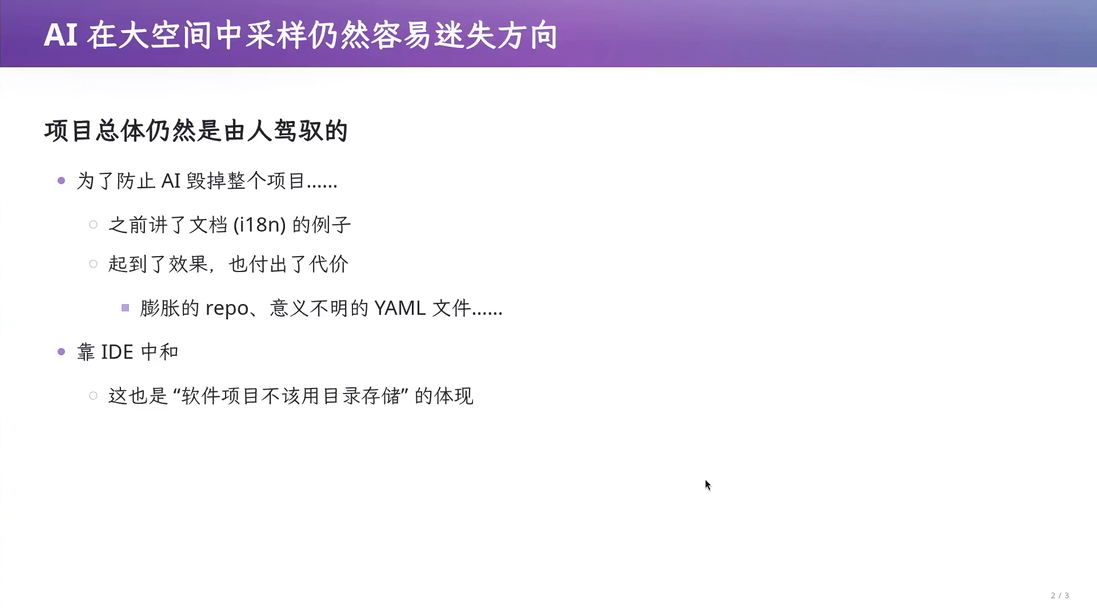
\includegraphics[width=0.92\textwidth]{figures/fig_35_ai_lost_in_large_space.png}
\caption{AI 在大空间中采样仍然容易迷失方向：以国际化（i18n）YAML 文件膨胀为例，揭示缺乏人类约束时 AI 局部最优导致的全局熵增，以及“软件项目不该仅用平面目录存储”的思考\vtag}
\end{figure}
\srcnote{01:18:15--01:18:30}

课堂以上一讲提到的\textbf{国际化多语言（i18n）规则}为例剖析了这一代价：为了防止 AI 在前端组件里硬编码中文或英文字符串，架构师定下一条铁律——“所有用户可见文案必须提取到独立的 YAML 语言包中”。这条规矩确实消除了硬编码，但也付出了沉重的代价：当成百上千次 AI 会话各自往仓库里塞入碎片的 YAML 键值时，仓库迅速膨胀出大量命名晦涩、语义重复、无人敢删的 YAML 文件！

为了压制这种系统性熵增，\texttt{dsh} 团队不得不维护了整整 \textbf{216 KB 的文字规矩（AGENTS.md 与各类 Skills 文档）}以及 \textbf{200 多个自动化检查脚本}。这也印证了蒋老师在前面课程中反复强调的洞见：\textbf{传统的文件系统目录树（Directory Tree）本质上是为人类手工编辑几十个文件设计的低维投影，根本不适合作为 AI 时代软件工程的底层存储抽象}；未来的 IDE 与代码库应当是带有强语义图索引与多视图投影的结构化数据库。

\subsection{本章小结}

本章通过对 \texttt{DeepSeek Harness} 仓库 117 天、22,395 次提交的深度考古，还原了它从最初 4 次创世提交（确立 \texttt{AGENTS.md} 与 vendoring 汇入 Cordis 框架）、前 10天构建可回放 Event Sourcing 会话，到 7 月底完成从终端 TUI 迈向 Web 浏览器甲板的完整演化史，并提炼出 \texttt{RFC -> ADR} 决策链等四大工程宝藏。

% =========================================================================
% SECTION 7
% =========================================================================
\section{生产“与人类对齐”的好代码：7 类 68 条工程门禁与架构契约}

既然 AI 在自由采样时会不可避免地产生代码退化（Slop）、破坏模块边界或留下思维链残渣，\texttt{DeepSeek Harness} 究竟是如何在工程流水线上把“坏代码”拒之门外的？答案是：\textbf{找到所有“不好”的特征，编写确定性的门禁规则将其强行排除——一旦检验失败，就打回让智能体重新采样（Rejection Sampling）！}（图 36）

\begin{figure}[H]
\centering
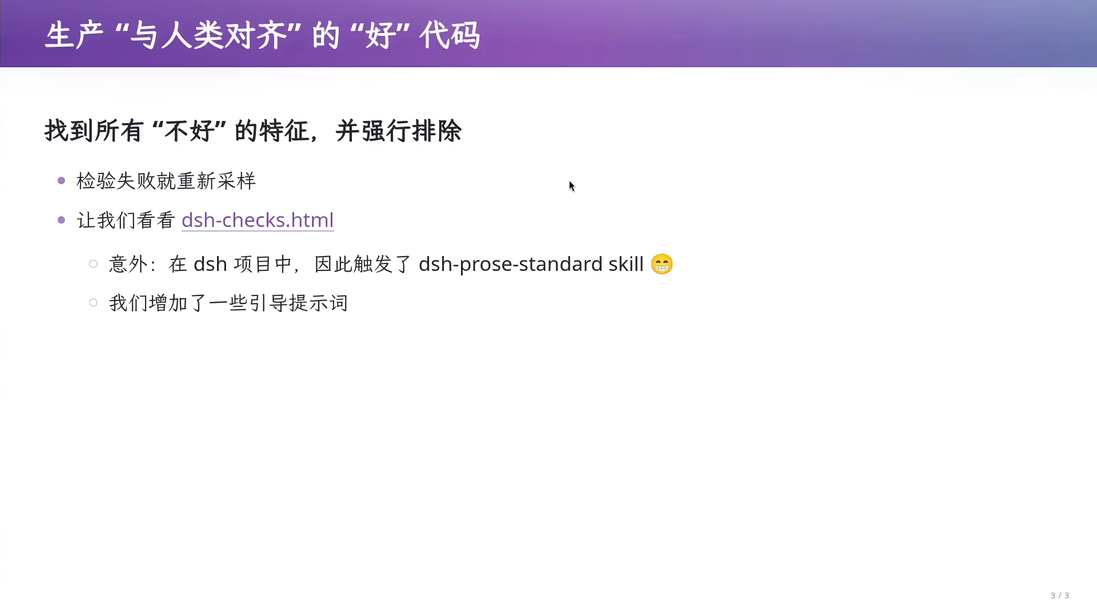
\includegraphics[width=0.92\textwidth]{figures/fig_36_good_code_gatekeeping.png}
\caption{生产“与人类对齐”的“好”代码：通过静态门禁检验失败即重新采样，并配套 \texttt{dsh-prose-standard} 技能消除文档中的思维链残留\vtag}
\end{figure}
\srcnote{01:20:15--01:20:30}

\subsection{\texttt{dsh-prose-standard} 技能：为什么严禁在代码注释里写“我们没有采用方案 C”？}

在检视代码门禁之前，蒋老师先分享了一个在 \texttt{dsh} 仓库中发现的极有意思的文档门禁技能——\textbf{\texttt{dsh-prose-standard}（配合 \texttt{dsh-trim-cot-leakage}）}。

当你让大模型修改一段代码并更新注释或文档时，AI 极喜欢把自己在推理阶段的\textbf{思维链残留（Chain-of-Thought Leakage）}写进代码注释里，例如：
\begin{quote}
\texttt{// 这里我们使用 Map 存储会话，而不是像之前那样使用 Array，也没有采用 WeakMap，因为需要支持序列化遍历……}
\end{quote}

一眼看去，这段注释似乎挺详细；但站在\textbf{软件演化的时间维度}上，这种注释是极其有害的毒药！为什么？因为三个月后，当另一位开发者阅读这段代码时，他只关心“当前这段代码是什么、遵守什么契约”；而注释里冒出的“没有采用旧方案 A、不采用方案 C”会凭空制造巨大的认知负担（旧方案 A 是什么？为什么要提它？）。更糟糕的是，当半年后代码又重构了，这句反向否定注释就会变成误导后来者的“幽灵历史残骸”。

因此，\texttt{dsh} 立下铁律：\textbf{“关于为什么放弃方案 B/C 的历史权衡，必须且只能写进冻结的 \texttt{ADR}（架构决策记录）文档中；而在源码注释、JSDoc 与产品文档里，只准正面陈述当前系统是什么（What it is），严禁出现思维链对比残留与反向否定句式！”}

\begin{lstlisting}[language={},caption={DeepSeek Harness 的 \texttt{dsh-prose-standard} 与 \texttt{dsh-trim-cot-leakage} 核心规范示意}]
# Rule: Trim Chain-of-Thought (CoT) Leakage in Code Comments & Docs
1. Describe the current state and invariant of the module directly.
2. NEVER leak conversational reasoning, revision history, or rejected alternatives
   into source comments or JSDoc (e.g., FORBIDDEN: "Instead of X, we now do Y",
   "We no longer use Z here", "Note that this does not use WeakMap").
3. Historical trade-offs and rejected options belong exclusively in immutable
   Architecture Decision Records (docs/adr/ADR-xxxx.md).
\end{lstlisting}

\begin{warningbox}{文档规范铁律：把“为什么不选 B”关进 ADR，让代码注释保持纯粹现在时}
在人机协同开发中，切忌任由 AI 将对话过程中的辩解与对比（如“这里我们不再使用数组，而是改用哈希表”）写入源码注释。源码注释只服务于描述当前状态的不变式（Invariants）；一切关于历史备选方案的否决理由都应归档于不可变的 \texttt{ADR} 文档中，从而避免代码再次演进后留下自相矛盾的“幽灵注释”。
\end{warningbox}

\subsection{7 类 68 条规则与三级拦截体系（\texttt{pre-commit} / \texttt{pre-push} / \texttt{CI}）}

为了全面展示 \texttt{dsh} 是如何把关每一次代码改动的，蒋老师把仓库中所有的检查脚本与规则整理成了交互式网页讲义 \texttt{dsh-checks.html}（图 37）。全库共有\textbf{7 大检查类别、68 条具体工程规则}，并按执行开销部署在三道防线上：毫秒级静态检查放在 \textbf{\texttt{pre-commit}}，包级编译与局部单测放在 \textbf{\texttt{pre-push}}（配有 \texttt{dsh-pre-push-checks} 技能），全量跨包集成验证与产物核验放在云端 \textbf{\texttt{CI}}。

\begin{figure}[H]
\centering

\includegraphics[width=0.92\textwidth]{figures/fig_37_dsh_checks_overview.png}
\caption{DeepSeek Harness《项目如何把关一次代码改动》全景（\texttt{dsh-checks.html}）：涵盖代码与类型质量、架构与依赖约束、行为正确性与回归、持久化与兼容性、文档与产品表达、构建交付与运行质量等 7 大类共 68 条规则\vtag}
\end{figure}
\srcnote{01:20:45--01:21:00}

课堂重点剖析了前两大类中最具代表性的工程门禁细则（图 38、图 39）：

\begin{figure}[H]
\centering
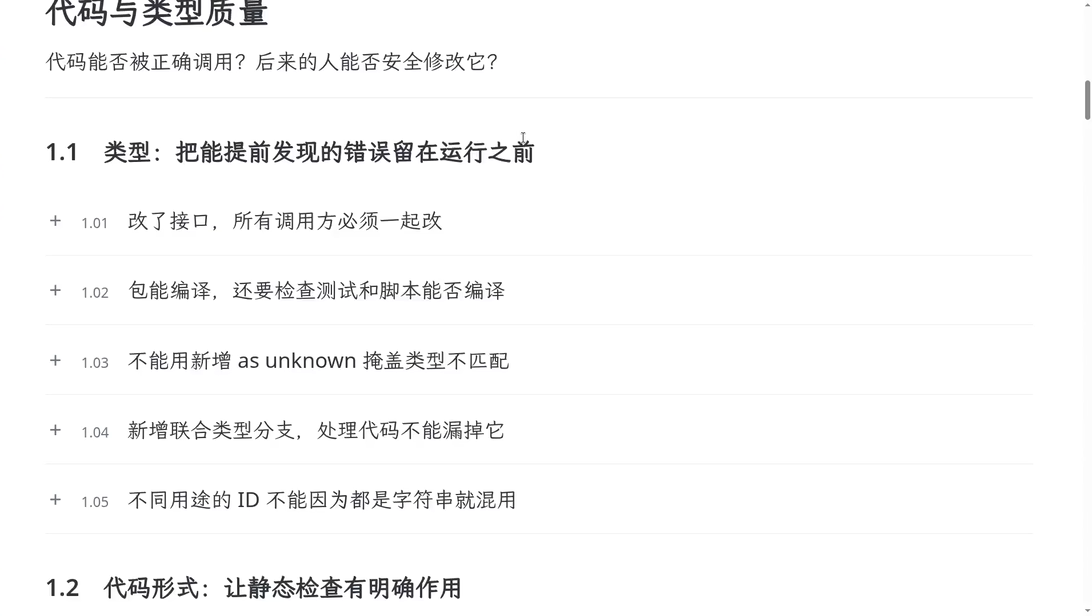
\includegraphics[width=0.92\textwidth]{figures/fig_38_dsh_checks_type_lint.png}
\caption{门禁细则（一）代码与类型质量：1.1 类型把关（改接口必改全调用方、检查测试与脚本编译、禁新增 \texttt{as unknown}、穷尽联合类型分支、Branded ID 防混用）与 1.2 静态检查规范\vtag}
\end{figure}
\srcnote{01:23:00--01:23:15}

\subsubsection{第一防线（1.1 \& 1.2）：类型检查前移与消除 AI 偷懒作弊}
\begin{enumerate}
    \item \textbf{严禁 \texttt{as any} 与新增 \texttt{as unknown} 掩盖类型不匹配（规则 1.03）}：
    用过 TypeScript 的同学都知道，当 AI 遇到复杂的泛型报错搞不定时，它最喜欢的“作弊大招”就是顺手写一个 \texttt{x as any}；如果你在 ESLint 里禁掉了 \texttt{any}，聪明反被聪明误的 AI 就会改写为双重强制转换 \texttt{x as unknown as TargetType} 来糊弄编译器！因此 \texttt{dsh} 专门编写了 AST 扫描门禁，严禁通过新增 \texttt{as unknown} 逃避类型检查。
    \item \textbf{构建产物与测试脚本全覆盖编译（规则 1.01 \& 1.02）}：
    必须先执行 \texttt{build:artifacts} 生成跨包类型声明，再执行全工作区 \texttt{build:check}，确保修改一个底层接口时，所有上层调用方、单元测试乃至构建脚本本身都必须同步通过类型检查；新增联合类型（Union Type）分支时，必须利用 \texttt{never} 穷尽性检查（Exhaustiveness Check）防止遗漏分支（规则 1.04）。
    \item \textbf{不同用途的 ID 必须使用 Branded Types（品牌化类型，规则 1.05）}：
    在智能体系统中，同时存在 \texttt{SessionId}、\texttt{MessageId}、\texttt{PluginId}、\texttt{WorktreeId} 等十几种标识符。在运行时它们虽然都是字符串（\texttt{string}），但如果直接声明为 \texttt{string}，AI 在传参时极易发生“把 \texttt{MessageId} 误传给需要 \texttt{SessionId} 的函数”的低级 Bug。通过引入 TypeScript \textbf{Branded ID}（如 \texttt{type SessionId = string \& \{ readonly \_\_brand: unique symbol \}}），即可在零运行时开销下利用编译器彻底杜绝跨业务 ID 混用！
    \item \textbf{严苛的 Lint 门禁（规则 1.2）}：
    所有异步 \texttt{Promise} 必须显式 \texttt{await} 或 \texttt{.catch()} 处理（严禁悬空 Promise）；严禁存在未使用的变量（Unused Variables，蒋老师结合自己当年写二重循环把内层 \texttt{j} 误写为 \texttt{i} 导致外层变量被静默覆盖的惨痛经历，强调该规则是捕获手误的第一利器）；所有非第三方导出的公共符号必须附带规范的 \texttt{JSDoc} 注释（由 \texttt{verify:export-jsdoc} 自动核验）。
\end{enumerate}

\begin{figure}[H]
\centering
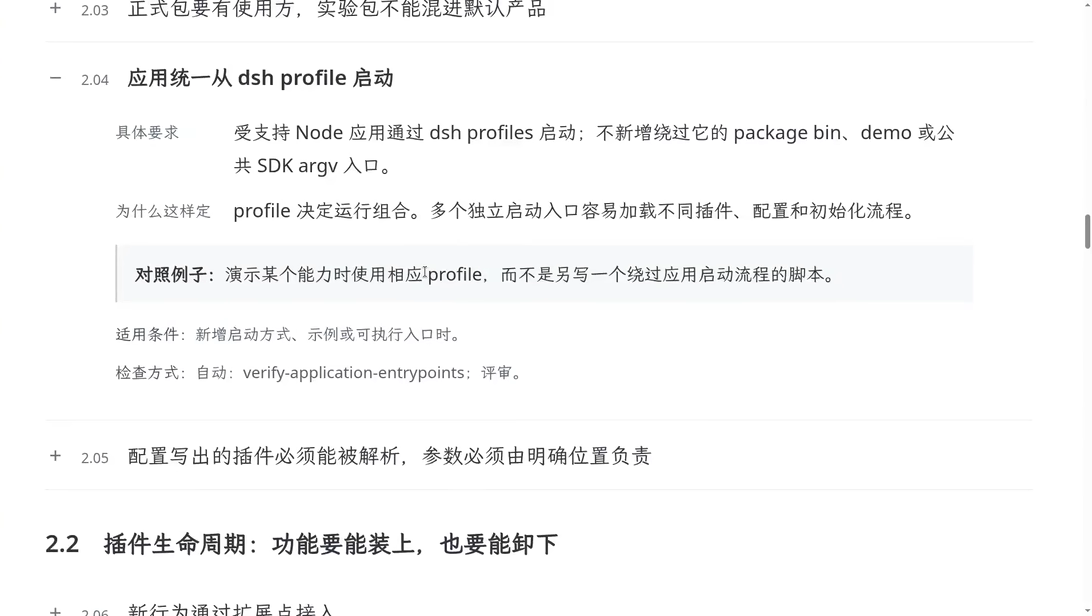
\includegraphics[width=0.92\textwidth]{figures/fig_39_dsh_checks_arch_boundary.png}
\caption{门禁细则（二）架构与依赖约束：正式包与实验包隔离（2.03）、应用统一从 \texttt{dsh profile} 启动（2.04，由 {\footnotesize\texttt{verify-application-entrypoints}} 自动核验）及插件可装可卸生命周期契约（2.2）\vtag}
\end{figure}
\srcnote{01:28:15--01:28:30}

\subsubsection{第二防线（2.1 -- 2.3）：架构边界、\texttt{dsh profile} 统一入口与插件生命周期}
\begin{enumerate}
    \item \textbf{应用统一从 \texttt{dsh profile} 启动（规则 2.04，图 39）}：
    当你想让 AI 写一个演示某个新能力的 Demo 时，AI 最容易偷懒的做法是在包目录下自己新建一个 \texttt{demo.ts} 脚本，手动 \texttt{import} 几个类拼凑运行。但这会导致严重的架构腐化：多个独立启动入口会加载不同的插件组合与初始化流程，久而久之没人知道系统真正的启动契约是什么。因此规则 2.04 强制规定：\textbf{所有受支持的 Node 应用与演示示例，必须统一通过 \texttt{dsh profiles} 启动，严禁新增绕过它的 \texttt{package bin}、\texttt{demo} 或公共 SDK \texttt{argv} 入口}，并由 {\footnotesize\texttt{verify-application-entrypoints}} 脚本自动拦截！
    \item \textbf{Cordis 插件生命周期——“功能要能装上，也要能卸下”（规则 2.2）}：
    微内核架构最核心的承诺是动态热插拔。如果一个插件在加载时注册了全局事件监听器、启动了后台定时器或向 DOM 树注入了按钮，但在卸载（Dispose）时没有清理干净，就会导致内存泄漏与幽灵回调。为此，\texttt{dsh} 编写了 \texttt{verify:runtime-closure}、\texttt{verify:client-domain-graph} 与 \texttt{verify:cordis-connect} 等一系列架构静态分析工具：强制所有跨模块交互必须走 Cordis 上下文总线；Waterfall 责任链钩子必须显式调用 \texttt{next()}；严禁客户端（Browser Client）代码直接依赖宿主（Node Host）内部实现或绕过 RPC 代理层。
\end{enumerate}

\begin{table}[H]
\centering
\small
\caption{DeepSeek Harness（\texttt{dsh-checks.html}）核心工程门禁规则与防御目标汇总表}
\begin{tabular}{p{2.1cm}p{2.9cm}p{4.0cm}p{4.2cm}}
\toprule
\textbf{规则编号与分类} & \textbf{门禁规则名称} & \textbf{主要防御的 AI 退化/工程腐化模式} & \textbf{自动化核验工具 / 手段} \\
\midrule
\textbf{1.01--1.02 类型} & 接口改动全量编译检查 & 改了底层接口却漏改测试脚本或边缘调用方 & \texttt{build:artifacts} + \texttt{build:check} \\
\textbf{1.03 类型安全} & 严禁新增 \texttt{as unknown} & AI 用 \texttt{as unknown as T} 双重强转掩盖类型错误 & AST 静态扫描门禁 \\
\textbf{1.05 领域建模} & Branded ID 防混用 & 把 \texttt{MessageId} 与 \texttt{SessionId} 等同类型字符串传反 & TypeScript Branded Types \\
\textbf{1.2 代码形式} & 公共导出强制 JSDoc & 新增公共 API 缺乏边界契约说明，破坏后续上下文 & \texttt{verify:export-jsdoc} \\
\textbf{2.04 架构入口} & 统一从 \texttt{dsh profile} 启动 & AI 私自新建绕过主初始化流程的独立 Demo 脚本 & {\footnotesize\texttt{verify-application-entrypoints}} \\
\textbf{2.2 插件周期} & 插件可装可卸与闭包隔离 & 跨包硬编码偷调函数、Waterfall 漏调 \texttt{next()}、卸载泄漏 & {\footnotesize\texttt{verify:runtime-closure} / \texttt{cordis-connect}} \\
\textbf{5.x 文档表达} & 剔除 CoT 思维链残留 & 在注释中写“不采用方案 B”等演化噪音误导读者 & \texttt{dsh-prose-standard} / \texttt{trim-cot-leakage} \\
\bottomrule
\end{tabular}
\end{table}

\subsection{本章小结}

本章深入拆解了 \texttt{DeepSeek Harness} 保障代码质量的工业级防线：从剔除注释中思维链残留的 \texttt{dsh-prose-standard} 技能，到涵盖 7 大类 68 条规则的 \texttt{dsh-checks.html} 门禁体系（Branded ID、禁 \texttt{as unknown}、\texttt{dsh profile} 统一启动、Cordis 插件可装可卸契约）。这套严密的自动化判别器（Verifier）将人类架构师的工程品味转化为了可执行的硬约束。

% =========================================================================
% SECTION 8
% =========================================================================
\section{表达“坏”容易，表达“好”很难：从 CEGIS、\texttt{unslop} 到递归自我改进（RSI）}

在领略了 \texttt{dsh} 宏大的 68 条工程门禁之后，课程在最后十分钟迎来了一次极具深度的哲学升华与反思：\textbf{既然我们可以靠不断添加“不准做 X、不准做 Y”的静态门禁和负面提示词来拦截坏代码，那么只要把负面规则加到一万条，AI 是不是就能自动涌现出顶级架构师的“好品味”了？}

蒋老师的回答斩钉截铁：\textbf{不能！因为“表达坏很容易，但表达好却极其困难；靠无穷叠加负面反例补丁，永远无法收敛到真正的最高品味！”}（图 40）

\begin{figure}[H]
\centering
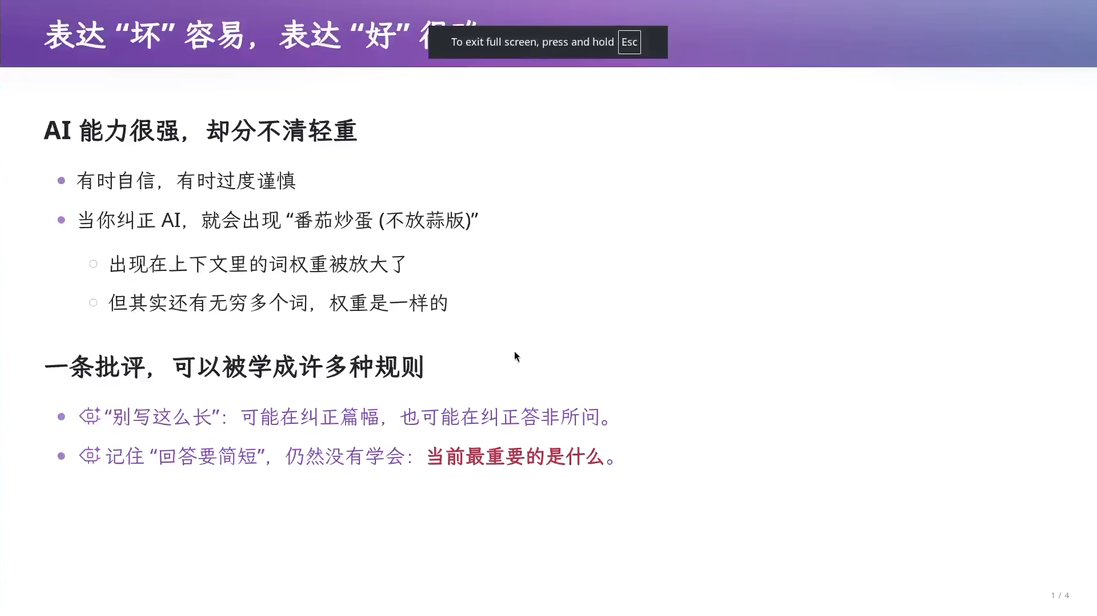
\includegraphics[width=0.92\textwidth]{figures/fig_40_bad_easy_good_hard.png}
\caption{表达“坏”容易，表达“好”很难：AI 能力虽强却分不清轻重，纠正 AI 时会出现“番茄炒蛋（不放蒜版）”的注意力权重放大效应\vtag}
\end{figure}
\srcnote{01:30:45--01:31:00}

\subsection{“番茄炒蛋（不放蒜版）”：注意力权重失衡与批评的歧义性}

为什么每当你纠正 AI 的一个具体小毛病，它的整体输出反而会变得越来越怪异？图 40 指出了大语言模型底层注意力机制（Self-Attention）的一个致命弱点——\textbf{AI 分不清轻重缓急}：
\begin{enumerate}
    \item \textbf{上下文词汇权重的病态放大（“番茄炒蛋不放蒜版”）}：
    假设你让 AI 做一道番茄炒蛋，它第一次做出来放了大蒜；你随口纠正了一句“番茄炒蛋不要放蒜”。对于人类厨师而言，“不放蒜”只是十几个隐含常识约束（不放香菜、不放芥末、不放巧克力……）中极其微不足道的一条，这些“不放 X”的权重本来都是零。但一旦“不要放蒜”这四个字显式进入了 Prompt 上下文，Transformer 的注意力机制就会赋予它极高的激活权重！结果 AI 不仅在炒菜时死盯着蒜，甚至在菜名、盘子装饰、菜谱文档和代码注释里到处写满\textbf{“这是一盘严格遵循无蒜架构规范的番茄炒蛋（No-Garlic Edition）”}！
    \item \textbf{一条批评可以被学成无数种表面规则}：
    当你对 AI 说“别写这么长！”时，你真正想表达的可能是“你答非所问、冗长繁琐没抓住重点”；但 AI 记住的表面规则却是机械的“字数截断 < 100 字”。下次遇到一个真正需要严谨分步推导的复杂架构问题时，它为了迎合“回答要简短”的死规矩，把关键边界条件全删光了——因为它始终没有学会\textbf{“在当前具体情境下，究竟什么才是最重要的”}。
\end{enumerate}

\subsection{CEGIS 反例引导归纳合成与无穷补丁不收敛定理}

从计算机科学理论来看，“靠不断报错打补丁来逼近目标程序”正是程序合成（Program Synthesis）领域的经典范式——\textbf{反例引导归纳合成（Counterexample-Guided Inductive Synthesis，简称 CEGIS）}（图 41）。

\begin{figure}[H]
\centering
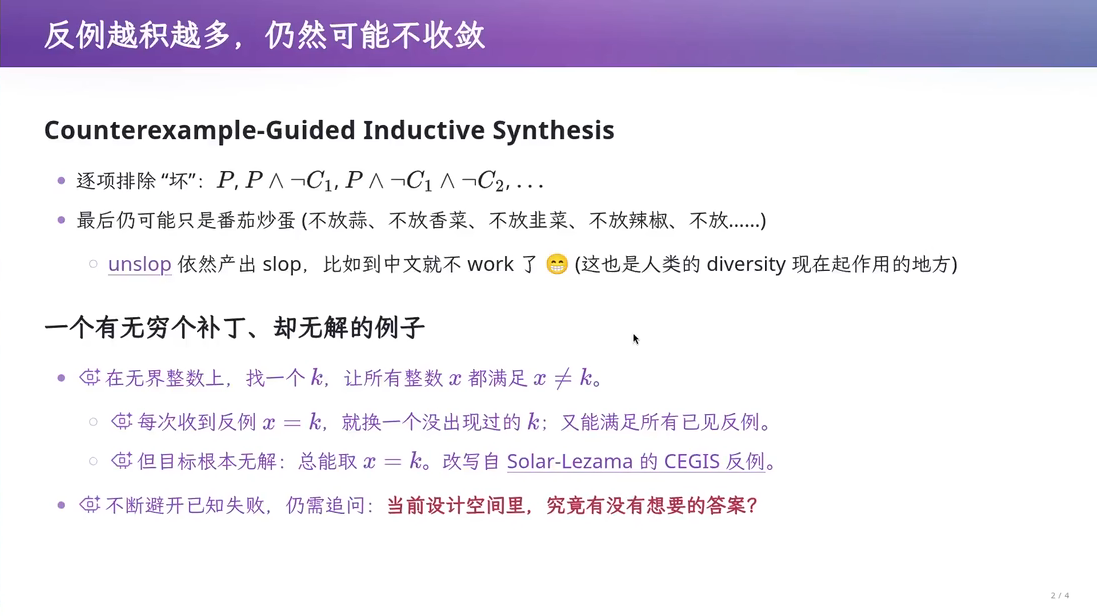
\includegraphics[width=0.92\textwidth]{figures/fig_42_cegis_counterexamples.png}
\caption{反例越积越多，仍然可能不收敛（Counterexample-Guided Inductive Synthesis，CEGIS）：逐项排除“坏”（$P \land \neg C_1 \land \neg C_2 \dots$）最后仍可能只是“不放蒜、不放香菜、不放韭菜、不放辣椒的番茄炒蛋”，改编自 Solar-Lezama 的经典无解反例\vtag}
\end{figure}
\srcnote{01:32:45--01:33:00}

蒋老师回顾道，这类程序合成技术在 2011年左右迎来了工业界的高光时刻——微软研究院的 Sumit Gulwani 在 POPL 2011 发表了著名的《Automating String Processing in Spreadsheets using Input-Output Examples》，成为后来家喻户晓的 \textbf{Excel FlashFill（智能快速填充）}功能。例如用户在 Excel 第一列输入电话号码 \texttt{025-12345678}，在第二列示范输入 \texttt{025}，合成器就能自动归纳出“提取连字符前的区号”程序；若遇到空格分隔的 \texttt{025 12345678} 失败了，用户再给一个反例，合成器就会打补丁修正规则。

然而，麻省理工学院（MIT）程序合成大师 Armando Solar-Lezama 在讲授 CEGIS 理论时曾给出过一个极具启发性的数学反例（图 41 下半部分）：如果合成器的假设空间（或偏好先验）选错了，单纯靠验证器不断抛出反例 $\neg C_i$，会出现**“打无穷多个补丁也永远无法收敛”**的病理现象！我们可以将其形式化为式 (5)：

\begin{equation}
\Phi_m(P) = P_0 \land \bigwedge_{i=1}^{m} \neg C_i(P), \qquad
f_m(x) = \begin{cases}
y_i^*, & \text{若 } x = c_i \;\; (i = 1, 2, \dots, m) \\
f_0(x), & \text{其他情况（未跳出错误基座 } f_0 \text{）}
\end{cases}
\end{equation}

其中各符号的数学与工程含义如下：
\begin{itemize}
    \item $P_0$（对应默认基座函数 $f_0(x)$）：智能体或程序合成器在初始偏置下采样的基准实现（如充满 AI 腔调的默认代码或错误结构的公式）；
    \item $C_i(P)$：第 $i$ 轮检验时触发的具体失败反例或静态门禁拦截条件（Counterexample，如 $x = c_i$ 时输出不符）；
    \item $\Phi_m(P)$：经过 $m$ 轮“检验失败—追加负面约束 $\neg C_i$”后累积的合取规范公式；
    \item $f_m(x)$：局部打补丁式的过拟合解（Overfitted Patching Solution）——例如课堂举例的目标是合成线性函数 $f^*(x) = x + 1$，当用户先后给出 $f(1)=2, f(2)=3, f(3)=4$ 以及一个特殊点 $f(4)=6$ 时，缺乏结构跃迁能力的合成器只会不断堆砌 \texttt{if (x == 4) return 6; else ...} 的特判分支；又如图 41 所示，若要在无界整数集 $\mathbb{Z}$ 上寻找一个整数 $k$ 使得对所有整数 $x$ 都满足 $x \neq k$，每当验证器给出反例 $x = c_i$，合成器只需挑一个没出现过的新整数 $k = \max_{1 \le i \le m} c_i + 1$ 即可骗过所有已见反例，但目标本身在当前设计空间中根本无解！
\end{itemize}

为了直观印证“反例黑名单在真实 AI 工程中的局限性”，蒋老师在课堂上打开了 Cursor 编辑器近期内置的爆款技能源码——\textbf{\texttt{unslop}（去除 AI 腔调与废话技能）}（图 42）：

\begin{figure}[H]
\centering
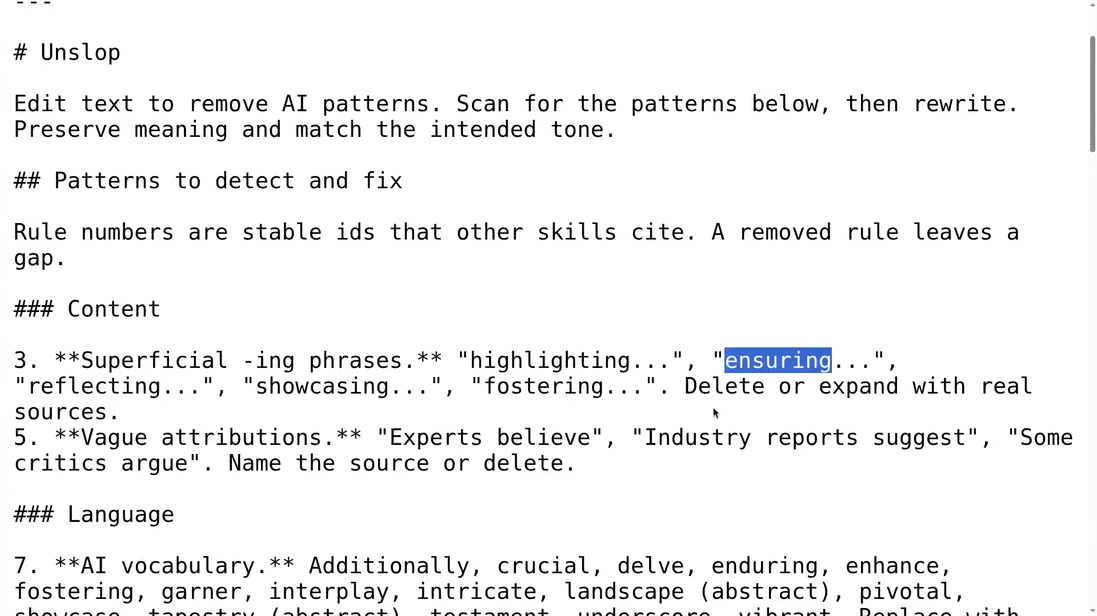
\includegraphics[width=0.92\textwidth]{figures/fig_43_cursor_unslop_skill.png}
\caption{Cursor 的 \texttt{unslop} 技能源码剖析：通过枚举 \texttt{highlighting...}、\texttt{ensuring...}、模糊归因（\texttt{Experts believe}）以及 \texttt{delve}、\texttt{crucial}、\texttt{tapestry}、\texttt{pivotal} 等高频 AI 词汇黑名单来过滤 AI 腔调\vtag}
\end{figure}
\srcnote{01:36:00--01:36:15}

\begin{lstlisting}[language={},caption={Cursor 内置 \texttt{unslop} 技能的典型反例黑名单规则摘录}]
# Unslop: Edit text to remove AI patterns. Scan for patterns below, then rewrite.
## Patterns to detect and fix
### Content
3. **Superficial -ing phrases.** "highlighting...", "ensuring...", "reflecting...",
   "showcasing...", "fostering...". Delete or expand with real sources.
5. **Vague attributions.** "Experts believe", "Industry reports suggest",
   "Some critics argue". Name the source or delete.
### Language
7. **AI vocabulary.** Additionally, crucial, delve, enduring, enhance, fostering,
   garner, interplay, intricate, landscape (abstract), pivotal, showcase,
   tapestry (abstract), testament, underscore, vibrant. Replace with plain words.
\end{lstlisting}

看着图 42 中密密麻麻的英文禁用词表（\texttt{delve}, \texttt{tapestry}, \texttt{pivotal}, \texttt{not just X, but Y}），蒋老师笑道：这就是最典型的\textbf{“番茄炒蛋不放蒜、不放香菜、不放韭菜、不放辣椒”}！当你用 \texttt{unslop} 把英文里的 \texttt{delve} 和 \texttt{tapestry} 全部禁掉之后，AI 换到中文语境下立刻又会造出“不仅……而且……”、“赋能”、“抓手”、“总而言之”等全新的中文 Slop；哪怕你把中英文词表都封杀干净，一篇没有禁用词但逻辑空洞、毫无洞见的文章，依然是彻头彻尾的 Slop！

\begin{knowledgebox}{程序合成理论启示：CEGIS 的归纳偏置边界与负面规则膨胀}
在反例引导归纳合成（CEGIS）中，验证器提供的反例 $\neg C_i$ 只能划掉搜索空间中的单个错误点。如果候选程序空间的先验分布（Inductive Bias）本身偏离目标，合成器就会退化为一张不断膨胀的 \texttt{if-else} 查找表（或像 \texttt{unslop} 一样枚举成百上千个禁用词），虽然在已知反例集上零失误，却永远无法泛化到未见的测试分布。
\end{knowledgebox}

\subsection{设计空间的跳跃：Luchins（1942）水罐实验与“蒸馏我自己”的 RSI 探索}

既然在错误的设计空间里修修补补（Local Modification）永远走不出死胡同，人类与未来的智能体该如何实现\textbf{“设计空间的跳跃（Jump in Design Space）”}？

课堂引入了格式塔心理学家亚伯拉罕·陆钦斯（Abraham S. Luchins）于 1942 年发表的经典认知心理学实验——\textbf{水罐实验（Water Jar Experiment，研究思维定势 Einstellung Effect）}（图 43）：

\begin{figure}[H]
\centering
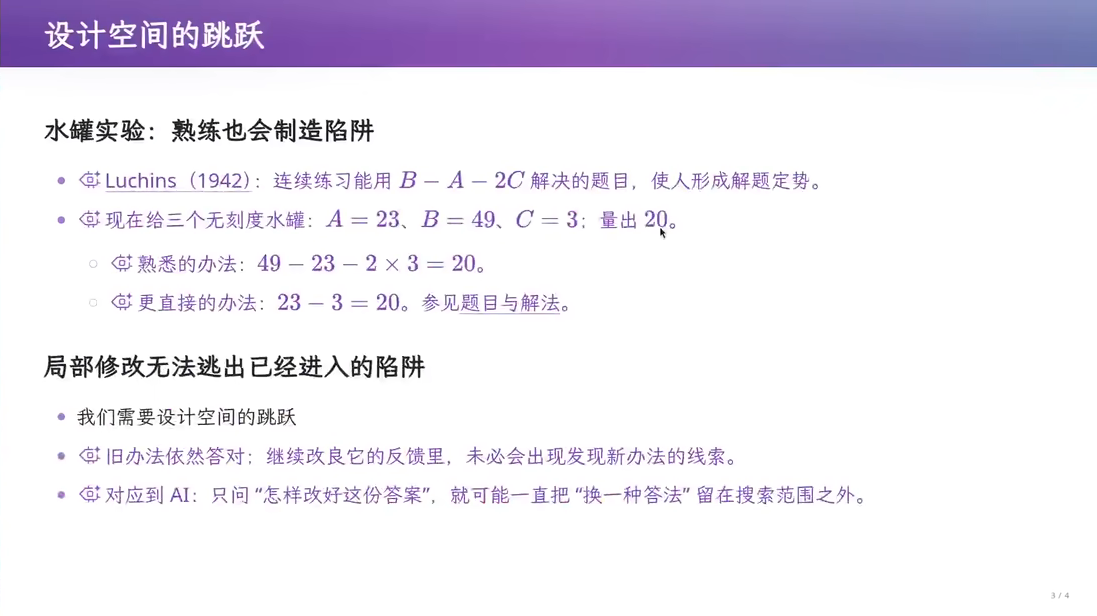
\includegraphics[width=0.92\textwidth]{figures/fig_41_luchins_water_jar.png}
\caption{设计空间的跳跃：Luchins（1942）水罐实验揭示“熟练也会制造陷阱”——局部修改无法逃出已经进入的思维定势，必须跳出当前搜索空间\vtag}
\end{figure}
\srcnote{01:39:45--01:40:00}

在 Luchins（1942）实验中，实验者给被试提供三个没有刻度的水罐 $A, B, C$，要求量出指定体积 $V^*$ 的水：
\begin{enumerate}
    \item \textbf{定势诱导阶段（前 5 题）}：例如第 2 题给定水罐容量 $A = 21,\; B = 127,\; C = 3$，要求量出 $V^* = 100$ 的水。被试很快发现可以通过“先把大罐 $B$ 装满，倒满一次 $A$，再倒满两次小罐 $C$”的固定三步套路精确得到 $127 - 21 - 2 \times 3 = 100$。连续做完 5 道同类题目后，被试对这套复杂公式变得无比熟练。
    \item \textbf{定势陷阱检验（第 6 题及后续题）}：接着给出图 43 中的题目——给定三个无刻度水罐 $A = 23,\; B = 49,\; C = 3$，要求量出 $V^* = 20$（或课堂口述的变体 $A=15, B=39, C=3$ 量出 $18$）。令人震惊的是，绝大多数刚刚经历过前 5 题训练的聪明人，依然毫不犹豫地端起大罐 $B=49$ 往外倒三次水，算出 $49 - 23 - 2 \times 3 = 20$；却完全看不见近在咫尺的一步极简解：直接把 $A=23$ 倒进 $C=3$，剩下的就是 $23 - 3 = 20$！
\end{enumerate}

我们将这一定势陷阱表达为如下多路径优化问题：

\begin{equation}
V_{\mathrm{habit}}(A, B, C) = B - A - 2C = 49 - 23 - 2 \times 3 = 20
\quad \text{vs.} \quad
V_{\mathrm{direct}}(A, C) = A - C = 23 - 3 = 20
\end{equation}

其中各符号的含义如下：
\begin{itemize}
    \item $A, B, C$：三个无刻度水罐的容积常数（在训练题中为 $A=21, B=127, C=3$；在测试题中为 $A=23, B=49, C=3$）；
    \item $V_{\mathrm{habit}}(A, B, C) = B - A - 2C$：局部改良定势路径（需要装水 1 次、倒出 3 次共 4 步操作）；值得注意的是，\textbf{旧办法在测试集上依然能答对（$49 - 23 - 6 = 20$ 完全通过单元测试！）}，因此在继续改良旧办法的局部反馈里，根本不会出现提示你切换到新办法的梯度线索；
    \item $V_{\mathrm{direct}}(A, C) = A - C$：跨设计空间跳跃后的全局最优路径（仅需 $23 - 3 = 20$ 一步倒水操作）。对应到 AI 辅助软件工程：\textbf{如果你只问 AI“怎样在这份旧代码上打补丁修好这个 Bug”，你就永远把“换一种架构答法”留在了搜索范围之外！}
\end{itemize}

在全课的压轴环节，蒋老师展示了他近期正在亲手做的一个前沿探索实验——\textbf{“蒸馏我自己（Distilling Myself）”}（图 44）：

\begin{figure}[H]
\centering
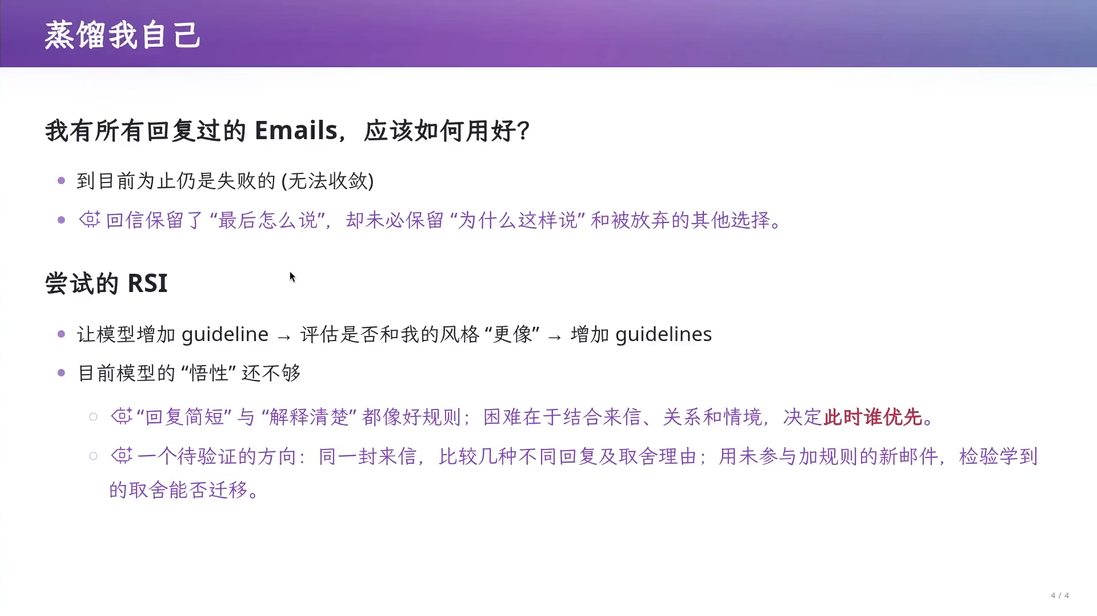
\includegraphics[width=0.92\textwidth]{figures/fig_44_distill_myself_rsi.png}
\caption{蒸馏我自己：利用主讲教师历史上所有回复过的真实 Emails 构建递归自我改进（RSI）闭环，探索从单点规则走向情境化优先级取舍\vtag}
\end{figure}
\srcnote{01:37:00--01:37:15}

蒋老师保存了自己过去十几年里回复学生、同行与合作伙伴的所有真实电子邮件（Emails），希望用这些高质量个人语料蒸馏出一个“能用蒋炎岩风格自动替我回邮件”的 Agent。然而实验过程中他发现了一个深刻的现象：
\begin{enumerate}
    \item \textbf{回信文本只保留了“最后怎么说”，却丢失了“为什么这样说”}：
    这与前面讲代码仓库需要 \texttt{ADR} 完全同构！静态的历史已发送邮件只展示了最终的文字结果，却没有记录面对这封来信时，作者脑子里原本浮现过哪几种回法、为什么放弃了长篇大论而选择了寥寥两句点拨。
    \item \textbf{尝试递归自我改进（Recursive Self-Improvement，RSI）及其瓶颈}：
    为了避免退化成 \texttt{unslop} 式的琐碎词表，蒋老师设计了一个 RSI 循环：\textbf{让模型根据预测回复与真实历史回复的差距（包括篇幅长度、句长分布、用词统计距离等可验证指标），每次不准针对单封邮件打特判补丁，而必须提炼出一条高层次的通用原则（General Guideline）写回 Skill，再去评估在验证集上是否离真实风格“更像”}。
    \item \textbf{为什么目前模型的“悟性”还不够？——缺乏元层次的情境优先级裁决}：
    实验到目前为止仍未完全收敛。原因在于，“回复应当简短有力”是一条好规则，“把复杂概念解释清楚”也是一条好规则；但当两条好规则在具体邮件面前发生冲突时，\textbf{人类真正的高品味在于结合来信者的身份、双方的熟悉关系与当前情境，在元层次（Meta-level）决定“此时此刻哪条规则优先”}。为此，蒋老师提出了下一步待验证的方向：针对同一封来信生成几种不同取向的回复并显式标注取舍理由，再用从未参与规则提炼的新邮件检验模型学到的“取舍权衡能力”能否真正泛化迁移。
\end{enumerate}

\begin{importantbox}{全讲终极升华：好品味不是“没有坏特征”，而是高维空间的取舍秩序}
回顾整堂课的脉络，从航母的百年演化、Linux 与 Python 的时间维度、SWE-bench 到 Taste-bench，再到 \texttt{DeepSeek Harness} 的 22,395 次提交与 68 条工程门禁，我们终于看清了 AI 时代软件工程的全貌：
\begin{itemize}
    \item \textbf{静态门禁与反例排除（CEGIS / \texttt{dsh-checks} / \texttt{unslop}）是造航母的底线护栏}：它们像航母上的操作手册与损管阀门一样，用确定性的规则兜住了系统的下限，防止 AI 在大空间采样中把项目毁掉。
    \item \textbf{设计空间跳跃与情境化权衡（Taste / \texttt{RFC->ADR} / RSI）是人类架构师的上限皇冠}：真正的“好代码”与“好架构”，绝不是靠一万条“番茄炒蛋不放蒜”的负面补丁拼凑出来的，而是在关键历史节点（如从运煤船跃迁到飞行甲板、从终端 TUI 跃迁到 Web 浏览器甲板）敢于跳出局部定势、并在相互冲突的工程目标之间做出优雅取舍的智慧结晶。
\end{itemize}
\end{importantbox}

\subsection{本章小结}

本章剖析了为何单纯依靠负面反例排除（CEGIS 局部补丁与 Cursor \texttt{unslop} 黑名单）会陷入“番茄炒蛋不放蒜”的注意力失衡与无穷补丁不收敛困境；结合 Luchins（1942）水罐实验与主讲教师“蒸馏我自己”的邮件回复 RSI 实验，指明了从局部修补迈向设计空间跳跃与情境化权衡元能力的未来方向。

% =========================================================================
% END OF NOTES SUMMARY
% =========================================================================
\newpage
\section*{全讲核心知识点与自检清单}

\begin{table}[H]
\centering
\small
\caption{第 10 讲《软件的演化（航母是怎么造出来的）》核心概念与工程方法速查表}
\begin{tabular}{p{3.0cm}p{4.5cm}p{5.8cm}}
\toprule
\textbf{知识模块} & \textbf{核心概念 / 历史坐标} & \textbf{生成式软件工程实战启示} \\
\midrule
\textbf{计算边界与平坦性} & ETH 亚指数计数、\texttt{PTIME} 复合闭包、诺特定理、生命之树退化为图 & 认识到人类数学工具偏爱对称平坦区域；用 AI 探索缺乏简洁闭包的复杂工程状态空间 \\
\textbf{能力证明与信号} & Spence（1973）信号理论、\texttt{Senior + Agent > Junior}、\textbf{AI Trajectory} & 静态成品已难区分人机贡献；积累不可伪造的 AI 交互日志（何时拒绝 AI、如何取证、如何进化） \\
\textbf{舰船百年演化史} & 1492 Santa Maria $\to$ 1811 New Orleans $\to$ 1922 Langley $\to$ 1945 Midway & 超级系统皆由微小增量 $+\Delta$ 演进而来；用 AI 大跨步探路验证 MVP，再回退用整舰工程标准重构 \\
\textbf{软件的时间维度} & Parnas（1972）信息隐藏、Linux 调度器更替 vs Python 2/3 十年迁移 & 将易变设计决定隐藏在模块边界后；用 \textbf{Git Rebase 冲突学习法}在极简内核上穿透历史例外 \\
\textbf{从解题到品味评测} & SWE-bench（3.79 $\to$ 65\%+）、Thurstone（1927）比较判断、\textbf{\texttt{Taste-bench}} & 二值验证的小事必被 RL 刷爆；通过多维成对比较与后续需求反转检验评估架构品味 \\
\textbf{DSH 演化考古} & 117 天 22,395 次提交、Cordis vendoring、Web 甲板跃迁、\texttt{RFC $\to$ ADR} & 先立 \texttt{AGENTS.md} 与微内核底座；用 RFC 对齐提案、用冻结式四段 ADR 保存被放弃方案的因果 \\
\textbf{好代码工程门禁} & \texttt{dsh-prose-standard}、7 类 68 条规则、Branded ID、\texttt{dsh profile} 统一入口 & 严禁注释残留思维链与反向否定句；将架构契约转化为 \texttt{pre-commit/pre-push/CI} 自动拦截脚本 \\
\textbf{从反例到空间跳跃} & CEGIS 不收敛反例、Cursor \texttt{unslop}、Luchins（1942）水罐定势、邮件 RSI & 负面黑名单只能兜底无法收敛到好品味；警惕局部修补定势，用含取舍理由的轨迹训练元判断力 \\
\bottomrule
\end{tabular}
\end{table}

\end{document}
